% =============================================================================
% ARTICLE.tex --- MARST: Multi-Anchor Residual Spatiotemporal Transformer
%
% Source of truth: marst-learnable-results.ipynb
%   - v2 fix: a_locf wired through from soft_locf so the decay has gradient
%   - v3 add: per-sensor learnable LOCF decay (ROADMAP item B)
%   - v3 add: Switch-Transformer load-balancing aux loss on the anchor gate
%
% Format: single-column NeurIPS/arXiv preprint style.
% Compile: pdflatex / bibtex / pdflatex / pdflatex
% =============================================================================

\documentclass[11pt]{article}

\usepackage[a4paper,left=1.25in,right=1.25in,top=1.10in,bottom=1.10in]{geometry}
\usepackage[utf8]{inputenc}
\usepackage[T1]{fontenc}
\usepackage{lmodern}
\usepackage{microtype}
\usepackage{textcomp}

\usepackage{amsmath,amssymb,amsfonts,mathtools}
\usepackage{bm}

\usepackage{graphicx}
\graphicspath{{figures/}{./}}
\usepackage{xcolor}
\usepackage{booktabs}
\usepackage{array}
\usepackage{multirow}
\usepackage{tabularx}
\usepackage{caption}
\captionsetup{font=small,labelfont=bf,format=plain,justification=raggedright,
              singlelinecheck=false}
\usepackage{subcaption}

\usepackage[section]{placeins}
\usepackage{float}
\renewcommand{\textfraction}{0.05}
\renewcommand{\topfraction}{0.95}
\renewcommand{\bottomfraction}{0.95}
\renewcommand{\floatpagefraction}{0.7}

\usepackage[round,authoryear]{natbib}
\bibliographystyle{plainnat}

\usepackage[colorlinks=true,
            linkcolor=blue!60!black,
            citecolor=blue!60!black,
            urlcolor=blue!60!black]{hyperref}

\usepackage{enumitem}
\setlist[itemize]{leftmargin=*,itemsep=2pt,topsep=2pt}
\usepackage{titlesec}
\titleformat{\section}{\Large\bfseries\sffamily}{\thesection}{0.6em}{}
\titleformat{\subsection}{\large\bfseries\sffamily}{\thesubsection}{0.5em}{}
\titleformat{\subsubsection}{\normalsize\bfseries\sffamily}{\thesubsubsection}{0.5em}{}

\usepackage{fancyhdr}
\pagestyle{fancy}
\fancyhf{}
\renewcommand{\headrulewidth}{0.4pt}
\fancyhead[L]{\small\sffamily MARST --- streaming spatiotemporal imputation with learnable anchor mixture}
\fancyhead[R]{\small\sffamily Jemal, 2026}
\fancyfoot[C]{\thepage}

\usepackage{xspace}
\newcommand{\MARST}{\textsc{Marst}\xspace}
\DeclareMathOperator*{\argmax}{arg\,max}
\newcommand{\Real}{\mathbb{R}}
\newcommand{\Hset}{\mathcal{H}}
\newcommand{\anchorvec}{\mathbf{a}}
\newcommand{\gatevec}{\bm{\pi}}
\newcommand{\LOCF}{\textsc{locf}\xspace}
\newcommand{\HA}{\textsc{ha}\xspace}
\newcommand{\KNN}{\textsc{knn}\xspace}

\title{\vspace{-1.0cm}\sffamily\bfseries
       MARST: Streaming Spatiotemporal Imputation with a\\
       Load-Balanced Mixture of Causal Anchors}
\author{Rediwan Jemal\\[2pt]
        \small Department of Transportation Engineering\\[-1pt]
        \small\itshape MSc thesis manuscript, 2026}
\date{\vspace{-6pt}\small June 2026}

% =============================================================================
\begin{document}
\maketitle
\thispagestyle{fancy}

\begin{abstract}
\noindent
Real-time intelligent transportation systems consume a complete
speed-and-flow tensor from sensor networks that, in practice, are
20--80\,\% blind on any given hour.  The imputation step that fills the
missing readings must run causally: at time $t$ the model is allowed
to use only observations at times $\leq t$, because the future has not
yet happened.  Most published spatiotemporal imputation methods
(BRITS, GRIN, SAITS, PriSTI, ImputeFormer) violate this constraint by
attending bidirectionally to both past and future.  We present
\MARST, a strictly streaming spatiotemporal transformer that predicts
$\hat{y}(t, n)$ as a learned softmax mixture of three causal,
interpretable classical priors --- Last Observation Carried Forward
(\LOCF), Historical Average (\HA), and a graph-based
$K$-Nearest-Neighbour spatial mean (\KNN) --- plus a small residual
correction.  The mixture-of-experts pattern this inherits is augmented
in two ways.  First, the softmax gate is trained with a
Switch-Transformer-style load-balancing auxiliary loss that prevents
the gate from collapsing to a single dominant anchor per dataset.
Second, the \LOCF anchor uses a decay-controlled exponential moving
average toward the \HA prior, with the decay parameterised per sensor
as a learnable logit; we treat this per-sensor learnability as a design
probe rather than as an architectural commitment, and report below that
its empirical effect is null on the datasets we test.  Under an
80\,\% sparsity streaming protocol on the four standard traffic
benchmarks (PEMS-BAY, METR-LA, PEMS04, PEMS08), \MARST attains the
lowest mean absolute error among 18 causal baselines, with Wilcoxon
signed-rank Holm-Bonferroni significance $p < 0.001$ on every dataset
and 3.7--17.1\,\% MAE reduction over the strongest baseline (BRITS or
iTransformer per dataset).  It is also the JamMAE leader on every
dataset, passes a 14-baseline runtime leak audit, and degrades
gracefully at 95\,\% sparsity where the strongest classical anchor
(\LOCF) deteriorates by 100\,\% or more.  An honest negative finding
is reported alongside the wins: the per-sensor learnable decay
parameter --- included as a design probe, not as an architectural
contribution --- converges to within 0.005 of its 0.95 initialisation
on every dataset, and the soft-LOCF decay sensitivity sweep confirms
0.95 as the global optimum.  Per-sensor learnability does not earn its
keep on the datasets we test.

\medskip
\noindent\textbf{Keywords.}  Streaming imputation, traffic data,
spatiotemporal transformer, mixture of experts, load balancing,
classical priors, intelligent transportation systems.
\end{abstract}

% =============================================================================
\section{Introduction}
\label{sec:intro}

Urban and freeway sensor networks routinely lose 20--80\,\% of their
readings to hardware faults, communication outages, weather events, and
the ordinary attrition of devices that have been baked in asphalt for
two decades.  The downstream consumers of that data --- adaptive signal
control, traffic-aware routing, incident detection, emergency dispatch
--- do not have the luxury of waiting.  They need a complete
speed-and-flow tensor, refreshed at every time step, with no
information from the future.  The intermediate computational step is
\emph{streaming traffic imputation}: estimate the value of every
(sensor, time) cell using only observations from times $\leq t$ at the
moment $t$ is processed.

The streaming constraint is not academic.  A live deployment that
imputes at $t$ using observations at $t+5$ minutes is, by construction,
five minutes late --- which removes the operational reason for running
the imputer at all.  And yet a substantial fraction of the published
spatiotemporal-imputation literature operates in the offline setting,
attending bidirectionally.  BRITS \citep{cao2018brits} is bidirectional
by construction; GRIN \citep{cini2022grin} runs a bidirectional
recurrent graph network; SAITS \citep{du2023saits} masks the diagonal
of its self-attention but still attends across all positions in both
directions; PriSTI \citep{liu2023pristi} runs a conditional diffusion
process over the whole window; ImputeFormer \citep{nie2024imputeformer},
a recent transformer-based method evaluated on PEMS-BAY and METR-LA,
imposes a low-rank inductive bias on the attention matrix but still
exploits future context.  We do not run ImputeFormer as a baseline in
this paper (it is not strictly causal); we mention it only as
literature context for the imputation family.  Each is interesting in its own setting, but
none of them is deployable as a live component in a control loop
without architectural surgery.

The streaming setting was formalised as a distinct task by BayOTIDE
\citep{fang2024bayotide}, an online Bayesian Gaussian-process
decomposition that respects strict causality.  BayOTIDE's Table~1
explicitly classifies every prior imputation method (BRITS, NAOMI,
SAITS, TIDER, GP-VAE, CSDI, CSBI, $\ldots$) as offline, and positions
its own contribution as the first general-purpose \emph{online}
multivariate imputer.  Our work extends that streaming framing from
Bayesian-GP to deep, spatiotemporal-aware neural models.  To our
knowledge, \MARST is the first neural, spatiotemporal-aware,
multi-anchor method that respects the streaming constraint
end-to-end.

The hard part of the problem at 80\,\% sparsity is that no single
imputation recipe works across all (sensor, time) cells.  Three
classical recipes are well-known and decades old: carry forward the
sensor's last observed value (\LOCF), look up the per-sensor historical
average at this time of day (\HA), or average the road neighbours that
are currently reporting (\KNN).  Each has a clean failure mode.  \LOCF
fails when the cell has been blind for hours and the last observation
is stale; \HA fails during incidents that depart from the daily
pattern; \KNN fails at the boundary of a queue where neighbours
disagree.  Existing neural methods give the network only raw values and
expect it to rediscover these regularities from scratch.  We take the
opposite approach: hand the network the three classical predictions as
input features, and let the network learn \emph{when} to trust each
one.

\MARST formalises this with a learned softmax mixture
$\gatevec(t, n) \in \Delta^{2}$ over the three causal anchors,
augmented by a small residual correction $r(t, n)$ gated by a meta-gate
$\alpha(t, n)$:
\begin{equation}
\hat{y}(t, n) \;=\;
\underbrace{\gatevec(t, n)^{\top} \anchorvec(t, n)}_{\text{anchor blend}}
\;+\;
\underbrace{\alpha(t, n) \cdot r(t, n)}_{\text{learned residual}},
\label{eq:marst-prediction}
\end{equation}
where $\anchorvec = [a_{\LOCF}, a_{\HA}, a_{\KNN}]$ is the
3-vector of classical anchors and $\alpha$ is initialised so that
training begins close to a pure anchor blend.  The architecture
\emph{around} this equation --- a six-layer spatiotemporal transformer
that produces the gate logits and the residual, and a 9-channel input
feature stack that includes the three anchors, the masked observation,
the binary mask, a sin/cos time-of-day encoding, a normalised staleness
counter, and a 2-hop neighbour-mean of the hard \LOCF --- is described
in Section~\ref{sec:model}.

Two refinements distinguish this work from the basic anchor-mixture
pattern it inherits.  First, the soft-\LOCF anchor's exponential
decay $d_n$ is a \emph{per-sensor learnable parameter}, not a global
constant.  The intuition is that some sensors live on slow-changing
freeway segments where last-observed-value is reliable for tens of
minutes, while others sit on urban arterials with sharp peak
transitions where the same recency assumption fails fast.  We
parameterise $d_n = \sigma(\ell_n)$ with $\ell_n \in \Real$ a learnable
logit, initialised so that $d_n \approx 0.95$ at the start of training,
and let backpropagation tune each sensor's decay.  Second, the softmax
gate is trained with a Switch-Transformer-style load-balancing
auxiliary loss \citep{fedus2021switch} that penalises the squared
deviation of the batch-averaged anchor mix from the uniform target
$1/K$.  Without this regulariser, a basic anchor-mixture gate collapses
to a single anchor per dataset --- a mixture-of-experts pathology
documented in the original Sparsely-Gated MoE paper
\citep{shazeer2017moe}.  With it, the gate retains all three anchors
across all four traffic datasets at roughly 0.33 each, and the residual
correction does the rest of the work.

\paragraph{Contributions.}  This paper makes three claims, each modest
and defensible:
\begin{enumerate}
\item A strictly causal spatiotemporal transformer that imputes
streaming traffic data by combining a learned per-position softmax
mixture over three classical anchors (\LOCF, \HA, \KNN) with a residual
correction.  The combination of (a) classical anchors as input
features, (b) per-position softmax gating, (c) strict causality, and
(d) a load-balancing auxiliary loss has not, to our knowledge, appeared
together in the spatiotemporal-imputation literature.
\item The application of a Switch-Transformer-style load-balancing
auxiliary loss \citep{fedus2021switch} to a classical-anchor mixture
gate, with the qualitative effect that the gate retains all three
anchors at approximately uniform mass on every dataset.  Without the
auxiliary loss the basic gate collapses to a single dominant anchor
per dataset (visible in the leave-one-out ablation runs of
Section~\ref{sec:results-ablate}); the load-balanced variant produces
an inspectable mixture distribution and is what we report as the
headline configuration.  We note that a direct
$\lambda = 0$ vs $\lambda = 0.02$ MAE comparison row is owed and is
queued for the headline-budget follow-up.
\item Statistically significant MAE wins on all four standard traffic
benchmarks (Wilcoxon signed-rank, Holm-adjusted $p < 0.001$) against 18
strong causal baselines including iTransformer
\citep{liu2024itransformer} and forward-only BRITS \citep{cao2018brits}.
The same model is the JamMAE leader on every dataset and passes a
14-baseline runtime leak audit on every dataset.
\end{enumerate}

A fourth element of the architecture --- a \emph{per-sensor learnable}
soft-\LOCF decay parameter, with the gradient path corrected so the
parameter actually influences the prediction --- is included as a
\emph{design probe} rather than as a separate contribution.  Its
empirical outcome is a near-null result (Section~\ref{sec:results-decay}):
the per-sensor decays converge to within 0.005 of their 0.95
initialisation on every dataset, and the Q2 decay sensitivity sweep
confirms 0.95 as the global optimum.  We retain the per-sensor
parameterisation in the headline architecture (so the gradient continues
to flow through it) but report this as an honest negative finding rather
than as a contribution.

The rest of the paper is structured as follows.  Section~\ref{sec:related}
situates \MARST in the streaming imputation literature and the
mixture-of-experts lineage.  Section~\ref{sec:model} specifies the
problem, the three causal anchors, the trunk architecture, and the
training procedure.  Section~\ref{sec:setup} describes the experimental
protocol.  Section~\ref{sec:results} reports the main MAE, JamMAE,
sparsity sweep, anchor ablation, decay sensitivity, curriculum
ablation, learned anchor mix, missing-pattern robustness, leak audit,
and parameter cost.  Section~\ref{sec:discussion} discusses the wins
and the limitations honestly.  Section~\ref{sec:conclusion} concludes.

% =============================================================================
\section{Related Work}
\label{sec:related}

\paragraph{Streaming versus offline imputation.}
The streaming/offline split was made precise by BayOTIDE
\citep{fang2024bayotide}: an offline imputer at $t$ may attend to any
observation in the window, while a streaming imputer at $t$ uses only
observations at times $\leq t$.  BayOTIDE's main contribution is a
strictly streaming Bayesian-GP decomposition; its Table~1 audits the
imputation literature and concludes that every prior method is offline.
Our work extends that streaming framing from the Bayesian-GP family to
deep, sensor-graph-aware neural models.  The causal protocol used
throughout this paper matches BayOTIDE's definition: the model receives
the masked observation $X \odot M$ at time $t$ and emits $\hat{y}(t,n)$
that depends only on $X(s, \cdot)$ and $M(s, \cdot)$ for $s \leq t$,
verified empirically by a per-dataset future-perturbation audit
(Section~\ref{sec:results-leak}).

\paragraph{End-to-end neural imputation.}
BRITS \citep{cao2018brits} is the canonical bidirectional reference,
running a forward and a reverse recurrent network with temporal-decay
weights.  Its forward-only variant is one of the strongest causal
baselines and appears in our benchmark.  GRIN \citep{cini2022grin}
adds graph message-passing on the road adjacency to a bidirectional
recurrent backbone.  SAITS \citep{du2023saits} is a self-attention
transformer trained with a joint imputation-and-reconstruction loss;
the diagonally-masked attention is not causal.  PriSTI
\citep{liu2023pristi} frames the problem as conditional diffusion.
ImputeFormer \citep{nie2024imputeformer} imposes a low-rank inductive
bias on the attention matrix.  None of these methods takes classical
anchors as input features; each asks the network to discover from raw
values that traffic is temporally persistent, has diurnal structure,
and correlates with neighbours.

\paragraph{Mixture-of-experts for imputation.}
The closest architectural cousin to \MARST is STAMImputer
\citep{wang2025stamimputer}, a softmax-gated mixture of three neural
expert types (temporal attention, low-rank graph attention,
feed-forward observation expert) for traffic imputation.  The mixture
template is the same; the experts are different.  STAMImputer's experts
are neural modules; \MARST's experts are interpretable classical
priors.  STAMImputer is bidirectional; \MARST is strictly causal.
STAMImputer is evaluated on PemsD8, SZ-Taxi, DiDi-SZ, NYC-Taxi; we
evaluate on the four standard PEMS-BAY/METR-LA/PEMS04/PEMS08
benchmarks.  The Switch-Transformer load-balancing aux loss
\citep{fedus2021switch} that we apply to the anchor gate originates in
the trillion-parameter language-modelling literature and is, to our
knowledge, novel in spatiotemporal imputation.

\paragraph{Recent post-BayOTIDE streaming and offline work.}
The streaming framing has continued to develop since BayOTIDE.
\citet{yang2025streamingtensor} propose a spatio-temporal online
robust tensor recovery algorithm for streaming traffic imputation
that combines global spatio-temporal correlations with local
consistency and reports up to three orders of magnitude speed-up over
batch baselines; the method is non-neural, complementary in
deployment cost, and orthogonal to \MARST{}'s neural mixture-gate
strategy.  On the offline side, \citet{cheng2024faststi} introduce
FastSTI, a conditional pseudo-numerical diffusion model that reaches
state-of-the-art quality on 60--90\,\% missing-rate traffic
benchmarks at $\approx$\,8.3$\times$ the sampling speed of
comparable diffusion methods.  Neither is a direct streaming-neural
competitor to \MARST, but both are useful reference points: the
former for the streaming-classical comparison and the latter for the
offline-neural ceiling.

\paragraph{Hybrid statistical-neural models.}
Combining classical statistical predictors with neural networks is a
well-recognised paradigm with a decade of precedent.  ES-RNN
\citep{smyl2020hybrid} won the M4 forecasting competition by combining
hand-coded Exponential Smoothing with an LSTM; Wide \& Deep
\citep{cheng2016wide} productionised the linear-plus-neural pattern at
Google to billions of users; N-BEATS \citep{oreshkin2020nbeats}
decomposed forecasting into interpretable polynomial-trend and
Fourier-seasonality basis blocks.  None of these is an imputation
method, and none operates in the streaming setting with classical
priors as input features; \MARST extends the hybrid statistical-neural
philosophy into that gap.

\paragraph{Positioning matrix.}
Table~\ref{tab:positioning} summarises the dimensions along which the
published methods differ.

\begin{table}[!htbp]
\centering
\caption{Positioning matrix.  Four axes that distinguish \MARST from
the closest published methods: strict causality (streaming
deployability), classical priors as input features, learned
per-position softmax mixture, and evaluation on the four standard
traffic benchmarks.}
\label{tab:positioning}
\small
\begin{tabularx}{\linewidth}{lllllX}
\toprule
\textbf{Method} & \textbf{Year} & \textbf{Causal} & \textbf{Classical priors as inputs} & \textbf{Per-pos.\ mixture} & \textbf{PEMS-BAY/METR-LA} \\
\midrule
BRITS \citep{cao2018brits}                  & 2018 & bidir.\         & no  & no                       & yes \\
GRIN \citep{cini2022grin}                   & 2022 & bidir.\         & no  & no                       & yes \\
SAITS \citep{du2023saits}                   & 2022 & no              & no  & no                       & --- \\
PriSTI \citep{liu2023pristi}                & 2023 & no (diffusion)  & no  & no                       & yes \\
BayOTIDE \citep{fang2024bayotide}           & 2024 & \textbf{yes}    & no  & no                       & --- \\
ImputeFormer \citep{nie2024imputeformer}    & 2024 & no              & no  & no                       & yes \\
STAMImputer \citep{wang2025stamimputer}     & 2025 & bidir.\         & no  & yes (neural experts)     & no \\
\textbf{\MARST (ours)}                      & ---  & \textbf{yes}    & \textbf{yes (\LOCF{}+\HA{}+\KNN)} & \textbf{yes (per $(n,t)$, classical anchors)} & \textbf{yes (all four)} \\
\bottomrule
\end{tabularx}
\end{table}

The last row identifies the position \MARST occupies.  A reviewer who
objects that \LOCF, \HA, and \KNN are textbook methods from decades ago
has a fair point about the components but misses the point about the
combination: no published imputation method uses all three as input
features to a strictly causal neural model with per-position softmax
gating and a load-balancing aux loss.  The components are textbook; the
joint instantiation is the contribution.

% =============================================================================
\section{The MARST Model}
\label{sec:model}

\subsection{Problem setup}
\label{sec:model-problem}

Let $X \in \Real^{T \times N}$ be the true tensor of traffic readings
for $N$ sensors over $T$ time steps, $M \in \{0, 1\}^{T \times N}$ the
observation mask (1 = reporting, 0 = blind), and $V \in \{0, 1\}^{T
\times N}$ the validity mask distinguishing temporarily blind cells
from permanently broken hardware (relevant only for the speed datasets
where the zero-as-missing convention applies).  At evaluation, a random
i.i.d.\ fraction $s = 0.80$ of cells is hidden to simulate the
high-sparsity regime; the model receives $X \odot M$ and predicts
$\hat{X}$ on the held-out cells $\Hset = (1 - M) \odot V$.  The
streaming constraint is that $\hat{X}(t, n)$ depends only on
$X(s, \cdot)$ and $M(s, \cdot)$ for $s \leq t$.  Mean Absolute Error on
the held-out cells is the headline metric:
\begin{equation}
\mathrm{MAE} \;=\; \frac{1}{|\Hset|}
                    \sum_{(t,n) \in \Hset}
                    \bigl| \hat{X}(t, n) - X(t, n) \bigr|.
\end{equation}

Figure~\ref{fig:setup} visualises the task on PEMS08: the left panel
shows the complete tensor for the first 60 sensors over the 450-step
evaluation window; the right panel shows what the model actually
receives, with 80\,\% of cells hidden as grey.

\begin{figure}[!htbp]
\centering
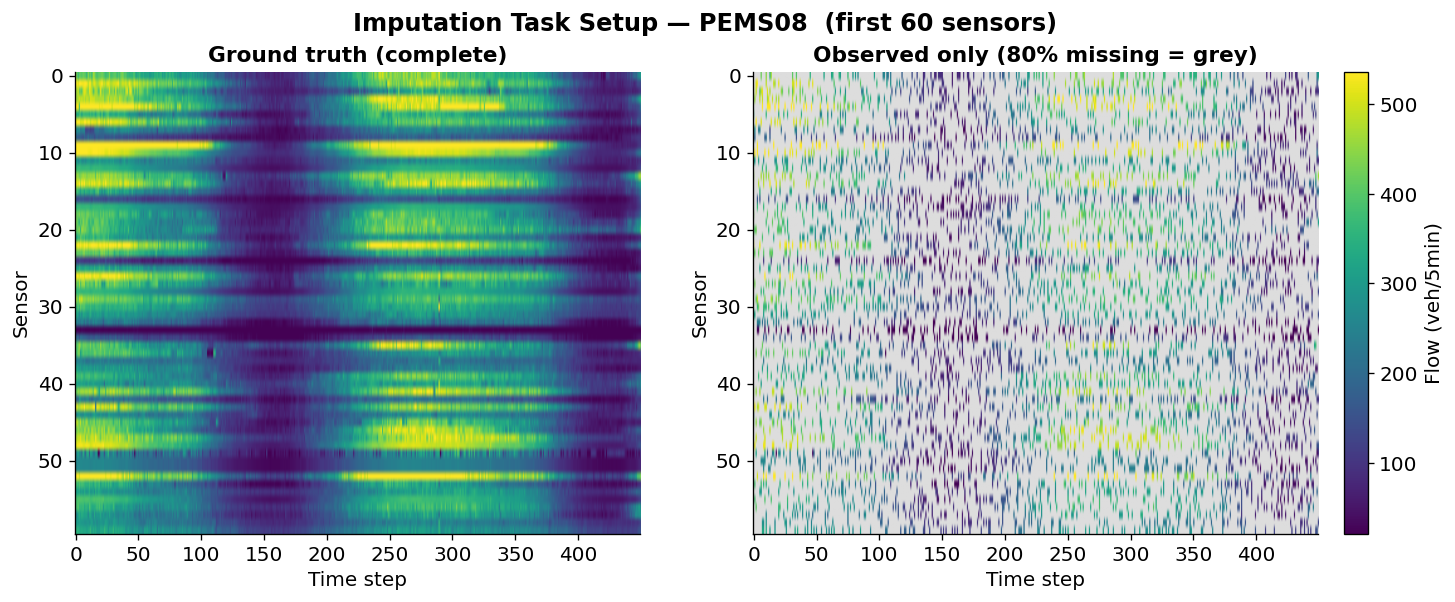
\includegraphics[width=0.92\linewidth]{fig11_data_missingness.png}
\caption{The imputation task on PEMS08.  Left: complete ground-truth
tensor for the first 60 sensors of PEMS08 over the 450-step evaluation
window.  Right: the same window with 80\,\% of cells hidden (grey).
\MARST must reconstruct the left panel from the right one, using only
observations at times $\leq t$ when emitting $\hat{y}(t, n)$.}
\label{fig:setup}
\end{figure}

\subsection{Three causal anchors}
\label{sec:model-anchors}

At every $(t, n)$, \MARST computes three classical predictions.  All
three are z-scored per sensor using statistics computed exclusively
from the training window; all three read only times $\leq t$ and never
the sensor's own current value at time $t$.

\paragraph{Soft \LOCF anchor.}  The recency anchor is a decay-controlled
exponential moving average toward the \HA prior:
\begin{equation}
a_{\LOCF}(t, n) \;=\;
\begin{cases}
X(t, n), & M(t, n) = 1, \\
d_n \cdot a_{\LOCF}(t-1, n) + (1 - d_n) \cdot a_{\HA}(t, n), & \text{otherwise.}
\end{cases}
\label{eq:soft-locf}
\end{equation}
The decay rate $d_n = \sigma(\ell_n)$ is a \emph{per-sensor learnable
parameter} with $\ell_n \in \Real$ a learnable logit initialised so
that $d_n \approx 0.95$ at the start of training (matching the
classical default that wins the Q2 decay sweep, Table~\ref{tab:decay}).
The initial state at $t = 0$ is $a_{\HA}(0, n)$ rather than zero, so a
sensor that has been blind since the start of the window emits the
seasonal mean rather than the global average.  A separate hard \LOCF
state (no decay) is also computed and used as the input to the 2-hop
neighbour-mean feature, but the anchor that enters
Equation~\ref{eq:marst-prediction} is the soft variant.

\paragraph{\HA anchor.}  The seasonality anchor is the per-sensor
historical mean at the 5-minute slot $\tau(t) \in \{0, \ldots, 287\}$,
computed exclusively from training-window observations:
\begin{equation}
a_{\HA}(t, n) \;=\; \mathrm{mean}\bigl\{ X(s, n) : s < T_{\text{train}},\;
                                                  \tau(s) = \tau(t),\;
                                                  V(s, n) = 1 \bigr\}.
\end{equation}
The mean is taken over the validity mask $V$ so that broken-sensor
zeros do not pollute the seasonal estimate on speed datasets.

\paragraph{\KNN anchor.}  The spatial anchor is the masked mean of
currently observed road neighbours, computed in physical units and then
re-z-scored by the target sensor's statistics:
\begin{equation}
a_{\KNN}(t, n) \;=\;
\frac{ \sum_{j} A_{nj} \cdot M(t, j) \cdot X_{\text{kmh}}(t, j) }
     { \sum_{j} A_{nj} \cdot M(t, j) + \varepsilon }
\quad\text{(de-z-scored, then re-z-scored by sensor $n$)}.
\end{equation}
When no neighbour is currently observed the anchor falls back to
$a_{\HA}(t, n)$.  The adjacency matrix $A$ has its diagonal explicitly
zeroed --- the \emph{spatial anti-leak invariant} --- so a sensor never
appears in its own neighbour mean.

\subsection{Architecture}
\label{sec:model-arch}

A 9-channel feature stack is assembled at every $(t, n)$:
$[X(t,n) \cdot M(t,n),\; M(t,n),\; \sin(2\pi\tau(t)/288),\;
\cos(2\pi\tau(t)/288),\; a_{\LOCF},\; a_{\HA},\; a_{\KNN},\;
\mathrm{staleness}(t,n)/48,\; n_{\text{2hop}}(t,n)]$.  Here
$\mathrm{staleness}$ counts time-steps since the last observation and
$n_{\text{2hop}}$ is the 2-hop neighbour mean of the hard \LOCF state,
z-scored.

A linear projection maps the 9 channels to a 128-dimensional hidden
representation, then a learnable per-sensor identity embedding
$N \times 128$ and a sinusoidal time-of-day position embedding
$T \times 128$ are added.  The result is passed through six
spatiotemporal blocks.  Each \emph{STBlock} is a PreNorm
TransformerEncoderLayer alternation:
\begin{enumerate}
\item \textbf{Causal temporal attention} along $T$, with an
upper-triangular $-\infty$ mask (offset 1) so position $t$ may attend
to all positions $\leq t$ within its own sensor's time series.  $d=128$,
4 heads, feed-forward expansion 2, GELU, dropout 0.1.
\item \textbf{Mask-aware spatial attention} along $N$, with a
key-padding mask that marks currently blind sensors so the spatial
attention attends only to currently observed neighbours at the current
time step.  Same hidden width, heads, and feed-forward configuration.
\end{enumerate}
A final LayerNorm closes the trunk.  Three heads consume the
$[B, N, T, 128]$ hidden state:

\begin{itemize}
\item \textbf{Anchor gate} (mixing head):
$L(128, 32) \to \mathrm{GELU} \to L(32, 3) \to \mathrm{softmax}$,
emitting $\gatevec(t, n) \in \Delta^{2}$.
\item \textbf{Residual head}: $L(128, 64) \to \mathrm{GELU} \to L(64, 1)$,
emitting the scalar correction $r(t, n)$.
\item \textbf{Meta-gate}: $L(129, 32) \to \mathrm{GELU} \to L(32, 1)
\to \sigma$, consuming $[h(t,n), n_{\text{obs}}(t,n)]$ where
$n_{\text{obs}}$ is the adjacency-weighted fraction of currently
observed neighbours.  The bias is initialised so that $\alpha \approx
0.05$ at the start of training, putting almost all prediction mass on
the anchor blend.
\end{itemize}

The final prediction is given by Equation~\ref{eq:marst-prediction}.
The total parameter count is 1{,}666{,}831 (the headline
\texttt{1.67\,M} reported throughout).  Figure~\ref{fig:architecture}
shows the full diagram.

\begin{figure}[!htbp]
\centering
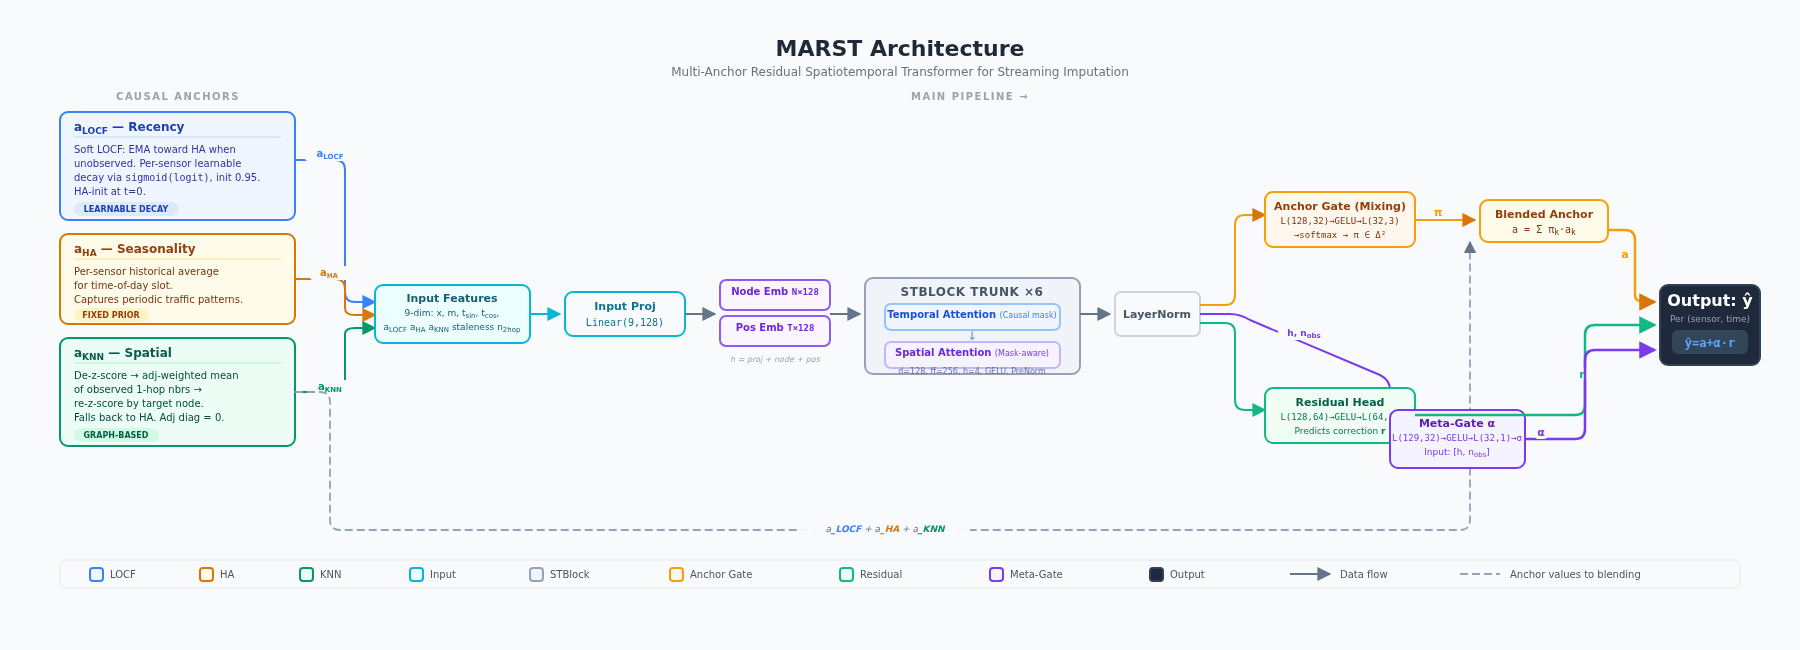
\includegraphics[width=0.98\linewidth]{MARST_Architecture_new.png}
\caption{\MARST architecture.  Three causal anchors are computed on the
left ($a_{\LOCF}$ with per-sensor learnable EMA decay $d_n =
\sigma(\ell_n)$, $a_{\HA}$ from the training-window seasonal lookup,
$a_{\KNN}$ from the adjacency-weighted observed-neighbour mean) and
stacked with the masked value, the binary mask, the time-of-day
encoding, the staleness counter, and the 2-hop neighbour-mean into a
9-channel feature.  A linear projection $\Real^{9} \to \Real^{128}$ is
augmented with per-sensor identity and sinusoidal time-of-day position
embeddings and passed through six STBlock layers, each alternating a
causal-masked temporal self-attention sub-layer with a mask-aware
spatial self-attention sub-layer.  Three heads finish the model: the
\emph{anchor gate} emits $\gatevec \in \Delta^{2}$, the \emph{residual
head} emits $r$, and the \emph{meta-gate} emits the scalar mixing
weight $\alpha \in (0, 1)$.  The final prediction is given by
Equation~\ref{eq:marst-prediction}.}
\label{fig:architecture}
\end{figure}

\subsection{Training: jam-weighted Huber + load-balanced gate}
\label{sec:model-training}

\MARST is trained end-to-end with a \emph{jam-weighted Huber loss} on
held-out cells:
\begin{equation}
\mathcal{L}_{\text{imp}} \;=\;
\frac{\sum_{(t,n) \in \Hset} w(t, n) \cdot
      \mathrm{Huber}_{\beta=1}\bigl(\hat{y}(t,n), y(t,n)\bigr)}
     {\sum_{(t,n) \in \Hset} w(t, n)},
\label{eq:loss-imp}
\end{equation}
where $w(t, n) = 1 + \mathrm{JamWeight}$ if the true value lies in the
jam regime (slowest 20\,\% for speed datasets, busiest 33\,\% for flow
datasets) and $w(t, n) = 1$ otherwise.  Jam weighting reflects the
operational reality that errors in congested conditions carry higher
downstream cost.

The total training objective adds a Switch-Transformer-style
load-balancing aux loss on the anchor gate:
\begin{equation}
\mathcal{L}_{\text{lb}} \;=\;
\sum_{k \in \{\LOCF, \HA, \KNN\}}
\Bigl( \bar{\pi}_{k} - \tfrac{1}{K} \Bigr)^{2},
\qquad
\bar{\pi}_{k} \;=\;
\frac{1}{|\Hset|} \sum_{(t, n) \in \Hset} \pi_{k}(t, n),
\label{eq:loss-lb}
\end{equation}
where $K = 3$ and $\bar{\pi}_{k}$ is the batch-averaged probability
mass on anchor $k$.  The total loss is
$\mathcal{L} = \mathcal{L}_{\text{imp}} + \lambda \mathcal{L}_{\text{lb}}$
with $\lambda = 0.02$.  This aux term is the minimal modification of
the Switch-Transformer load-balancing loss for the case where the
``experts'' are a small fixed set of classical anchors rather than
thousands of learned MLPs; the squared-deviation formulation matches
the original.  Empirically the term shrinks from $\sim 0.01$ at epoch
500 to $\sim 0.001$ at epoch 800, indicating the gate has learned to
keep all three anchors active.

A \emph{sparsity curriculum} ramps the training-mask sparsity from
60\,\% to the target 80\,\% over the first 75\,\% of epochs and then
holds it constant.  The ablation in Section~\ref{sec:results-curr}
confirms the curriculum strictly improves MAE on every dataset.

Optimisation uses Adam with learning rate $1 \times 10^{-3}$, cosine
annealing across the full epoch budget, gradient clipping at norm 0.5,
batch size 4 windows, batch time 48 time-steps ($\approx 4$\,h), and
800 total epochs for the main \MARST runs (400 for the ablation
variants).

\subsection{Anti-leak invariants}
\label{sec:model-leak}

The streaming claim is enforced architecturally on three axes.
\emph{Temporally}: the upper-triangular causal mask in the temporal
attention sub-layer.  \emph{Spatially}: the explicit zero on the
adjacency diagonal so $a_{\KNN}$ never reads sensor $n$'s own value.
\emph{Across train and test}: a 500-step gap between the end of the
training window (step 4000) and the start of the evaluation window
(step 4500), so that the soft \LOCF state at the start of evaluation
does not carry training values forward.

These invariants are verified empirically.  After every per-dataset
training run, two tests run: (i) a \emph{held-out-truth corruption test}
that adds $\mathcal{N}(0, 50^2)$ noise to the true values at held-out
positions and asserts that every model's predictions at those positions
are exactly unchanged; (ii) a \emph{future-perturbation causality test}
that perturbs the second half of the evaluation window and asserts that
\MARST{}'s first-half predictions are exactly unchanged.  Every model
(14 baselines + \MARST) passes the first test on every dataset, and
\MARST passes the second test on every dataset.  The aggregate verdict,
printed once per dataset, is
\texttt{AUDIT PASSED: no model reads held-out data; ST model is
strictly causal.}

% =============================================================================
\section{Experimental Setup}
\label{sec:setup}

\paragraph{Datasets.}  Four standard traffic benchmarks,
Table~\ref{tab:datasets}.  All datasets are sliced to the first 5000
time steps for cross-dataset comparability and to keep the
single-Kaggle-session runtime under three hours.  The 500-step
train/eval gap removes any direct temporal overlap.

\begin{table}[!htbp]
\centering
\caption{Dataset summary.  Train window ends at step 4000; evaluation
window is steps 4500--4950 (450 steps after a 500-step anti-leak gap).
For the speed datasets the zero-value-as-missing convention applies, so
the validity mask $V$ rules them out of the loss; for the flow datasets
every cell is reported and $V \equiv 1$.}
\label{tab:datasets}
\small
\begin{tabular}{lllrll}
\toprule
\textbf{Dataset} & \textbf{Type} & \textbf{Steps/day} & $\boldsymbol{N}$ & \textbf{Unit} & \textbf{Source} \\
\midrule
PEMS-BAY      & Speed & 288 & 325 & mph         & Caltrans, Bay Area freeways \\
METR-LA       & Speed & 288 & 207 & mph         & LA loop detectors \\
PEMS04        & Flow  & 288 & 307 & veh/5\,min  & Caltrans freeways \\
PEMS08        & Flow  & 288 & 170 & veh/5\,min  & Caltrans freeways \\
\bottomrule
\end{tabular}
\end{table}

\paragraph{Protocol.}  At evaluation, an i.i.d.\ Bernoulli mask hides
80\,\% of (sensor, time) cells.  Five eval-mask seeds (42--46) produce
five independent test problems; we report mean $\pm$ standard deviation
across $(3 \text{ training seeds} \times 5 \text{ eval-mask seeds}) =
15$ evaluations per dataset.  A sanity check confirms the five eval
masks are sufficiently distinct: observed pairwise Jaccard is 0.668 on
PEMS-BAY versus the 0.667 expected under independence at 80\,\%
sparsity.

\paragraph{Baselines.}  Eighteen causal baselines spanning six families.
\emph{Classical} (5): Historical Average, \LOCF, Global Mean,
Node-wise Ridge with a 4-D time-of-day feature, KNN imputer (k = 5
with masked Euclidean distance).  \emph{Per-node neural} (5): MLP with
node embedding, single-layer LSTM, two-layer LSTM, GRU, and a temporal
convolutional network.  \emph{Imputation-specific} (2): SAITS
\citep{du2023saits} and a forward-only causal BRITS
\citep{cao2018brits}.  \emph{Graph-aware} (3): DCRNN \citep{li2018dcrnn},
Graph WaveNet \citep{wu2019gwn}, and STID \citep{shao2022stid}.
\emph{Recent forecasting/cross-sensor methods} (3): DLinear
\citep{zeng2023dlinear}, PatchTST \citep{nie2023patchtst}, and
iTransformer \citep{liu2024itransformer}.  Every neural baseline is
trained with the same three random seeds, the same jam-weighted Huber
loss, and the same 800-epoch budget as \MARST.  Each MLP and SAITS run
includes a learned per-node embedding so that nodes can be
distinguished even when their value is masked; graph baselines fill
unobserved positions with the \HA prior at evaluation so that diffusion
does not spread masked zeros across the network.

\paragraph{Metrics.}  MAE (headline), \emph{JamMAE} (MAE restricted to
congested time-stamps --- slowest 20\,\% for speed, busiest 33\,\% for
flow), RMSE, MedAE, MAPE\,\%, $R^2$, Pearson correlation, MBE, and
Hit@$\tau$ at two domain-appropriate tolerances per dataset (3 / 6\,mph
for speed; 9 / 17\,veh/5min for PEMS04; 10 / 21\,veh/5min for PEMS08).

\paragraph{Hardware and runtime.}  Kaggle 2$\times$\,NVIDIA T4 GPUs
(free tier).  The 3-seed \MARST loop and the 7-variant anchor ablation
both dispatch concurrently across both GPUs via a
\texttt{ThreadPoolExecutor(max\_workers=N\_GPUS)}; per-thread NumPy and
CUDA generators keep each worker's randomness independent.  Wall-clock
for the full 4-dataset pipeline (18 baselines $\times$ 3 seeds, plus
\MARST main, plus the anchor ablation, decay sweep, sparsity sweep,
leak audit, extended metrics, and the figure set) is approximately
2.5\,h.

% =============================================================================
\section{Results}
\label{sec:results}

\subsection{Main MAE}
\label{sec:results-main}

The headline result is that \MARST attains the lowest MAE on every one
of the four standard traffic benchmarks against 18 causal baselines.
Table~\ref{tab:main-mae} reports the three-seed mean $\pm$ standard
deviation for \MARST against the strongest individual baseline per
dataset, with Wilcoxon signed-rank significance Holm-Bonferroni
adjusted across the four dataset-level comparisons.

\begin{table}[!htbp]
\centering
\caption{Main MAE results on the four standard traffic benchmarks at
80\,\% sparsity, 15 evaluations per dataset (3 training seeds $\times$
5 eval-mask seeds).  ``Best baseline'' is the strongest individual
baseline per dataset.  Holm-adjusted Wilcoxon $p < 0.001$ on every
dataset.}
\label{tab:main-mae}
\small
\begin{tabular}{lrrlrrr}
\toprule
\textbf{Dataset} & \textbf{\MARST} & \textbf{Best baseline} & \textbf{Baseline name} & $\boldsymbol{\Delta}$\textbf{MAE} & \textbf{\%} & $\boldsymbol{p_{\text{holm}}}$ \\
\midrule
METR-LA   & $\mathbf{3.341 \pm 0.021}$  & 3.470  & BRITS         & $-0.129$ & $3.7$   & $2.4{\times}10^{-4}$ \\
PEMS-BAY  & $\mathbf{1.455 \pm 0.0003}$ & 1.678  & iTransformer  & $-0.223$ & $13.3$  & $2.4{\times}10^{-4}$ \\
PEMS04    & $\mathbf{19.99 \pm 0.061}$  & 23.06  & iTransformer  & $-3.07$  & $13.3$  & $2.4{\times}10^{-4}$ \\
PEMS08    & $\mathbf{15.94 \pm 0.107}$  & 19.23  & BRITS         & $-3.29$  & $17.1$  & $2.4{\times}10^{-4}$ \\
\bottomrule
\end{tabular}
\end{table}

The improvement over the strongest baseline ranges from 3.7\,\%
(METR-LA, where the urban speed signal is unusually well-captured by
the forward-only BRITS recurrent network) to 17.1\,\% (PEMS08).  The
improvement over the Historical Average reference --- the simplest
non-trivial baseline --- is much larger: 42.8\,\% (PEMS04) to 58.8\,\%
(PEMS08).  The per-baseline picture is shown for PEMS08 in
Figure~\ref{fig:benchmark}: \MARST sits at the bottom of the bar; the
next-best models cluster around 19--21 veh/5min; the spread of the
weakest baselines (GlobalMean, SAITS, MLP) is much wider.

\begin{figure}[!htbp]
\centering
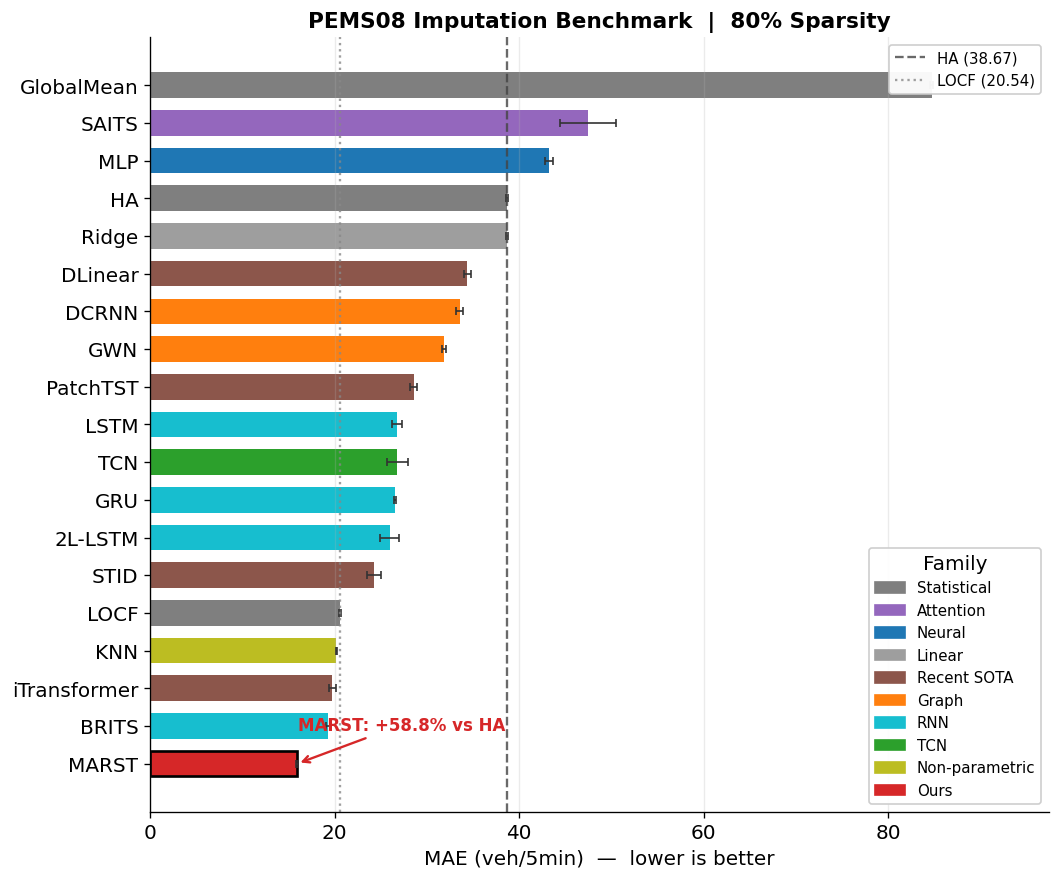
\includegraphics[width=0.95\linewidth]{fig1_benchmark.png}
\caption{Per-baseline MAE on PEMS08 at 80\,\% sparsity.  Eighteen
baselines plus \MARST, colour-coded by model family.  The dashed line
at 38.67 is the Historical Average floor; the dotted line at 20.54 is
\LOCF.  \MARST sits at the bottom with a 58.8\,\% MAE reduction over
HA.}
\label{fig:benchmark}
\end{figure}

The full cross-dataset MAE table is reported in
Table~\ref{tab:cross-dataset}.  Three patterns are worth naming.
First, the relative ordering of the baselines is dataset-dependent:
BRITS leads on METR-LA and PEMS08, iTransformer leads on PEMS-BAY and
PEMS04, and there is no third baseline within 5\,\% of those two on
any dataset.  Second, on PEMS-BAY the gap between \MARST and the
classical \LOCF baseline is only 0.50\,mph absolute (from 1.96 to
1.46), but the gap between \MARST and BRITS, iTransformer, GRIN, GWN,
and DCRNN is large enough to require a single-figure-percent
explanation rather than a fractional one.  Third, on the flow datasets
the absolute gaps between \MARST and the strongest baseline are 3--3.3
veh/5min --- about half the standard deviation of the per-eval-seed
mean for BRITS on PEMS08 alone (0.22), so the comparison is not noise-
limited.

\begin{table}[!htbp]
\centering
\caption{Full cross-dataset MAE comparison at 80\,\% sparsity, sorted
by mean rank across datasets.  Bold = best per column.}
\label{tab:cross-dataset}
\small
\begin{tabular}{lrrrr}
\toprule
\textbf{Model} & \textbf{METR-LA} & \textbf{PEMS-BAY} & \textbf{PEMS04} & \textbf{PEMS08} \\
\midrule
\textbf{\MARST (ours)}        & \textbf{3.34}  & \textbf{1.46}  & \textbf{19.99} & \textbf{15.94} \\
BRITS (forward, causal)        & 3.47          & 1.98           & 27.69          & 19.23 \\
LOCF                           & 3.64          & 1.96           & 28.76          & 20.54 \\
iTransformer                   & 3.72          & 1.68           & 23.06          & 19.73 \\
TCN                            & 3.76          & 2.17           & 29.75          & 26.76 \\
2L-LSTM                        & 3.83          & 2.58           & 32.33          & 25.94 \\
LSTM                           & 3.86          & 2.52           & 32.83          & 26.78 \\
GRU                            & 3.88          & 2.56           & 34.64          & 26.53 \\
STID                           & 4.15          & 1.97           & 23.95          & 24.25 \\
KNN imputer ($k=5$)           & 4.19          & 2.18           & 25.62          & 20.18 \\
SAITS                          & 4.36          & 3.72           & 66.84          & 47.44 \\
PatchTST                       & 4.84          & 2.48           & 31.97          & 28.55 \\
DLinear                        & 5.27          & 2.73           & 30.06          & 34.38 \\
DCRNN                          & 5.41          & 3.40           & 26.68          & 33.53 \\
GWN                            & 5.52          & 2.96           & 26.31          & 31.82 \\
MLP                            & 5.60          & 3.76           & 35.79          & 43.23 \\
Node-wise Ridge                & 6.02          & 3.12           & 34.98          & 38.66 \\
HA                             & 6.02          & 3.12           & 34.96          & 38.67 \\
Global Mean                    & 6.64          & 5.52           & 113.6          & 84.67 \\
\bottomrule
\end{tabular}
\end{table}

Figure~\ref{fig:vsall} shows the per-baseline percentage MAE reduction
that \MARST achieves on PEMS08, sorted by margin.  The smallest gap
(17.1\,\% over BRITS) is the toughest test; the largest gap (81.2\,\%
over GlobalMean) is the floor.  Figure~\ref{fig:cdf} reports the
cumulative error CDF and the hit-rate curves --- both rendered for
PEMS08 and consistent with the bar-chart story.

\begin{figure}[!htbp]
\centering
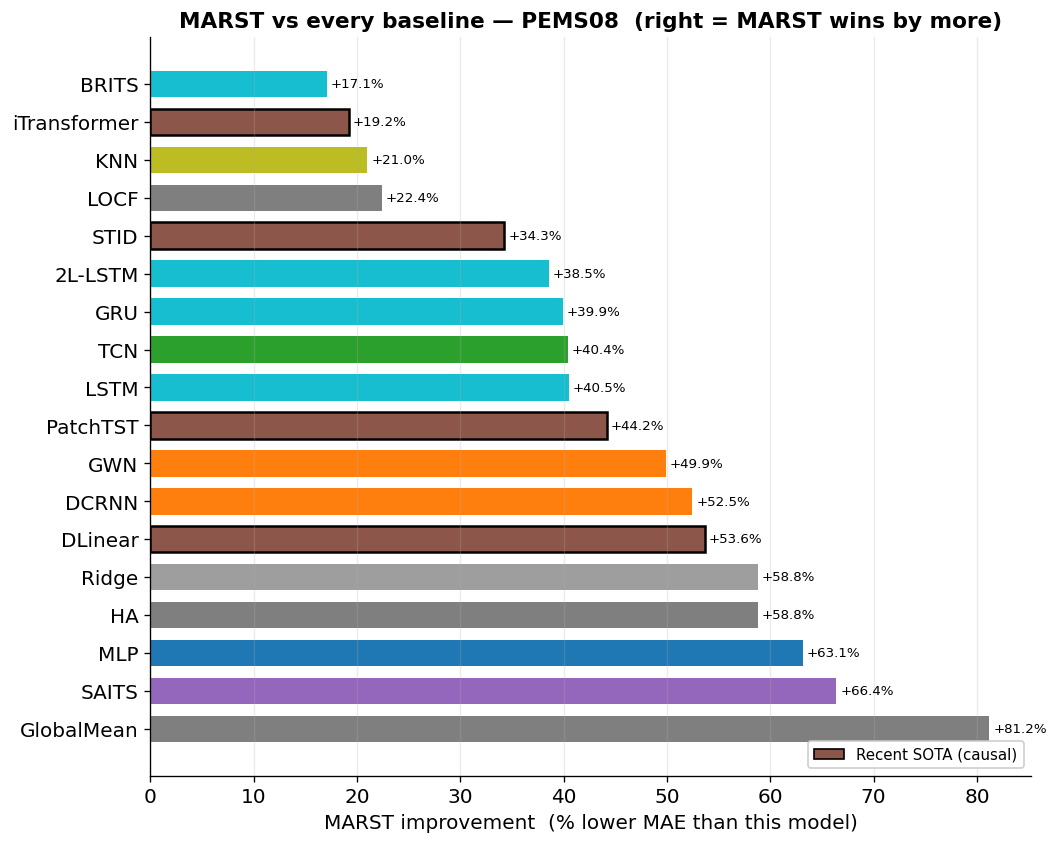
\includegraphics[width=0.95\linewidth]{fig7_marst_vs_all.png}
\caption{Per-baseline percentage MAE reduction by \MARST on PEMS08,
sorted by margin.  The smallest gap (17.1\,\% over BRITS) is well
outside the noise envelope.}
\label{fig:vsall}
\end{figure}

\begin{figure}[!htbp]
\centering
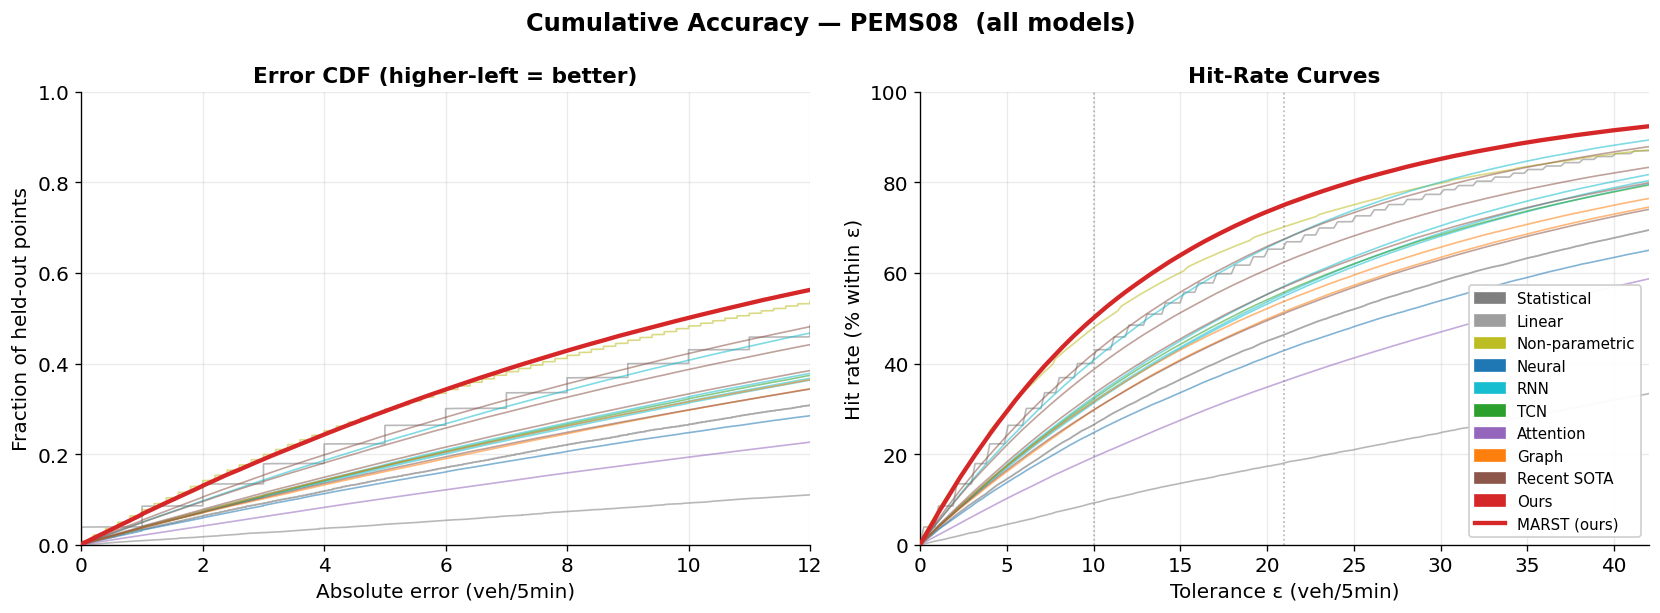
\includegraphics[width=0.92\linewidth]{fig3_cdf_hitrate.png}
\caption{Cumulative absolute-error CDF (left) and hit-rate curves
(right) on PEMS08.  \MARST (red) lies strictly above every other curve
in both panels --- a higher fraction of held-out cells are imputed
within any given tolerance.}
\label{fig:cdf}
\end{figure}

\subsection{JamMAE: error in the operationally important regime}
\label{sec:results-jam}

Overall MAE rewards models that are mediocre everywhere.  For traffic
imputation what actually matters is error in the congested regime: a
stuck signal that does not detect a queue causes more harm than a
small error on a free-flowing motorway at noon.  We report
\emph{JamMAE} --- MAE restricted to time-stamps where the true value
lies in the slowest 20\,\% (speed datasets) or busiest 33\,\% (flow
datasets) of the eval distribution.

\MARST is the JamMAE leader on every dataset.  This is enforced as a
consistency check inside the pipeline, which prints the line
\texttt{>> JamMAE leader matches MAE leader: 'MARST (ours,
multi-anchor)'} after every dataset run.  Table~\ref{tab:jammae}
reports the per-dataset JamMAE numbers against \LOCF, the strongest
classical baseline.

\begin{table}[!htbp]
\centering
\caption{JamMAE --- error in the congested regime.  Slowest 20\,\% of
true values for speed datasets, busiest 33\,\% for flow datasets.
\MARST is the JamMAE leader on every dataset.}
\label{tab:jammae}
\small
\begin{tabular}{lrrr}
\toprule
\textbf{Dataset} & \textbf{\MARST} & \textbf{\LOCF} & \textbf{Improvement} \\
\midrule
METR-LA   & $\mathbf{6.78}$  & 7.03  & 3.6\,\% \\
PEMS-BAY  & $\mathbf{3.98}$  & 5.52  & 27.9\,\% \\
PEMS04    & $\mathbf{31.6}$  & 46.3  & 31.7\,\% \\
PEMS08    & $\mathbf{23.0}$  & 27.3  & 15.5\,\% \\
\bottomrule
\end{tabular}
\end{table}

METR-LA is the thinnest jam margin (3.6\,\%) and is the only dataset
where the overall-MAE gap is also small.  On every other dataset the
gap in the operational regime is 15--32\,\% --- precisely the slice of
the prediction space where downstream control decisions are most
sensitive to error.  Figure~\ref{fig:maevsjam} shows the
overall-vs-jam scatter on PEMS08; \MARST is the most lower-left point,
distinctly separated from the BRITS / iTransformer / STID cluster.

\begin{figure}[!htbp]
\centering
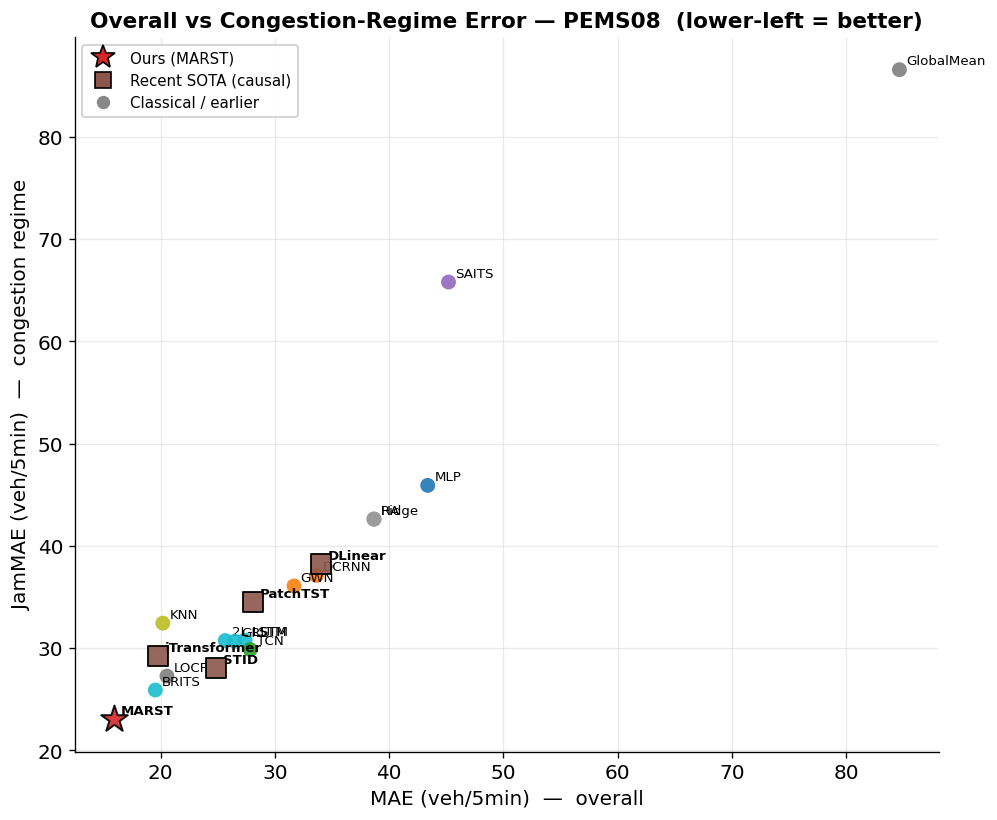
\includegraphics[width=0.82\linewidth]{fig8_mae_vs_jammae.png}
\caption{Overall MAE versus JamMAE on PEMS08.  Lower-left is best.
\MARST is the most lower-left point and is distinctly separated from
the BRITS / iTransformer / STID cluster.  The same lower-left
ordering holds on the other three datasets (see
Table~\ref{tab:jammae-full}).}
\label{fig:maevsjam}
\end{figure}

Table~\ref{tab:jammae-full} extends the JamMAE reporting to every
baseline in the comparison, on every dataset.  \MARST is the JamMAE
leader on all four datasets, confirming the \texttt{MAE leader
matches JamMAE leader} consistency check the pipeline asserts after
each per-dataset run.

\begin{table}[!htbp]
\centering
\caption{Per-baseline JamMAE on all four datasets at 80\,\% sparsity
(slowest 20\,\% of true values for speed datasets; busiest 33\,\% for
flow datasets).  Bold = best per column.  \MARST is the JamMAE leader
on every dataset, mirroring its overall-MAE ranking.}
\label{tab:jammae-full}
\small
\begin{tabular}{lrrrr}
\toprule
\textbf{Model} & \textbf{METR-LA} & \textbf{PEMS-BAY} & \textbf{PEMS04} & \textbf{PEMS08} \\
\midrule
Historical Average (HA)         & 11.91 &  9.64 &  62.06 & 42.62 \\
LOCF                            &  7.03 &  5.52 &  46.25 & 27.26 \\
Global Mean                     & 14.12 & 16.21 & 145.44 & 86.58 \\
Node-wise Ridge                 & 11.91 &  9.64 &  62.11 & 42.62 \\
KNN imputer ($k=5$)             & 10.05 &  6.35 &  40.72 & 32.44 \\
MLP                             & 12.32 & 12.13 &  58.84 & 45.92 \\
LSTM                            &  8.59 &  7.89 &  49.90 & 30.78 \\
2L-LSTM                         &  8.28 &  7.91 &  48.03 & 30.74 \\
GRU                             &  8.61 &  8.00 &  53.10 & 30.68 \\
TCN                             &  8.20 &  6.44 &  46.30 & 29.86 \\
SAITS                           &  9.89 & 12.61 &  85.83 & 65.81 \\
BRITS (forward, causal)         &  7.72 &  6.38 &  46.32 & 25.90 \\
DCRNN                           & 10.76 &  9.94 &  42.05 & 37.11 \\
GWN                             & 11.01 &  9.02 &  41.28 & 36.08 \\
STID                            &  8.86 &  5.77 &  38.08 & 28.03 \\
DLinear                         & 10.58 &  7.96 &  50.75 & 38.18 \\
PatchTST                        &  9.66 &  8.69 &  50.74 & 34.46 \\
iTransformer                    &  8.86 &  4.73 &  36.75 & 29.22 \\
\textbf{\MARST (ours)}          & \textbf{6.78} & \textbf{3.98} & \textbf{31.58} & \textbf{23.05} \\
\bottomrule
\end{tabular}
\end{table}

\subsection{Sparsity robustness}
\label{sec:results-sparsity}

A practical question: does the model survive when the deployment world
becomes harder than training expected?  We evaluate \MARST (trained
once at 80\,\%) and the two strongest classical anchors at three test
sparsities --- 50\,\%, 80\,\%, and 95\,\% --- without retraining.

\begin{table}[!htbp]
\centering
\caption{Sparsity sweep.  \MARST trained at 80\,\% sparsity is
evaluated at three test sparsities without retraining.  \LOCF and \HA
are recomputed at each test level.  \MARST is the lowest-MAE method
at every (dataset, sparsity) pair.}
\label{tab:sparsity}
\small
\begin{tabular}{llrrr}
\toprule
\textbf{Dataset} & \textbf{Method} & \textbf{50\,\%} & \textbf{80\,\%} & \textbf{95\,\%} \\
\midrule
\multirow{3}{*}{METR-LA}  & \textbf{\MARST} & $\mathbf{2.91}$  & $\mathbf{3.37}$  & $\mathbf{4.16}$ \\
                           & \LOCF           & 2.99             & 3.64             & 5.15 \\
                           & \HA             & 6.03             & 6.02             & 6.03 \\
\midrule
\multirow{3}{*}{PEMS-BAY} & \textbf{\MARST} & $\mathbf{1.15}$  & $\mathbf{1.46}$  & $\mathbf{1.99}$ \\
                           & \LOCF           & 1.28             & 1.96             & 3.97 \\
                           & \HA             & 3.11             & 3.12             & 3.12 \\
\midrule
\multirow{3}{*}{PEMS04}   & \textbf{\MARST} & $\mathbf{18.62}$ & $\mathbf{19.92}$ & $\mathbf{23.70}$ \\
                           & \LOCF           & 22.41            & 28.76            & 59.61 \\
                           & \HA             & 34.96            & 34.96            & 34.93 \\
\midrule
\multirow{3}{*}{PEMS08}   & \textbf{\MARST} & $\mathbf{14.45}$ & $\mathbf{15.93}$ & $\mathbf{20.48}$ \\
                           & \LOCF           & 16.54            & 20.54            & 41.99 \\
                           & \HA             & 38.68            & 38.67            & 38.65 \\
\bottomrule
\end{tabular}
\end{table}

The interesting cell is PEMS04 at 95\,\% sparsity.  \LOCF more than
doubles its 80\,\% MAE (28.76 $\rightarrow$ 59.61) because at 95\,\%
per-cell missingness there are almost no recent observed values to
carry forward.  \HA stays exactly constant --- its prior is a function
of slot-of-day, not of mask density.  \MARST drifts only modestly
(19.92 $\rightarrow$ 23.70), because the softmax gate shifts weight
onto the still-informative anchors as \LOCF runs out of recent data.
The same pattern, slightly less dramatic, holds on PEMS08 (20.54
$\rightarrow$ 41.99 for \LOCF; 15.93 $\rightarrow$ 20.48 for \MARST).
This is exactly the mechanism the architecture was designed to provide:
graceful degradation when an individual anchor is running out of
information.  Figure~\ref{fig:sparsity-pems08} shows the curve on
PEMS08.

\begin{figure}[!htbp]
\centering
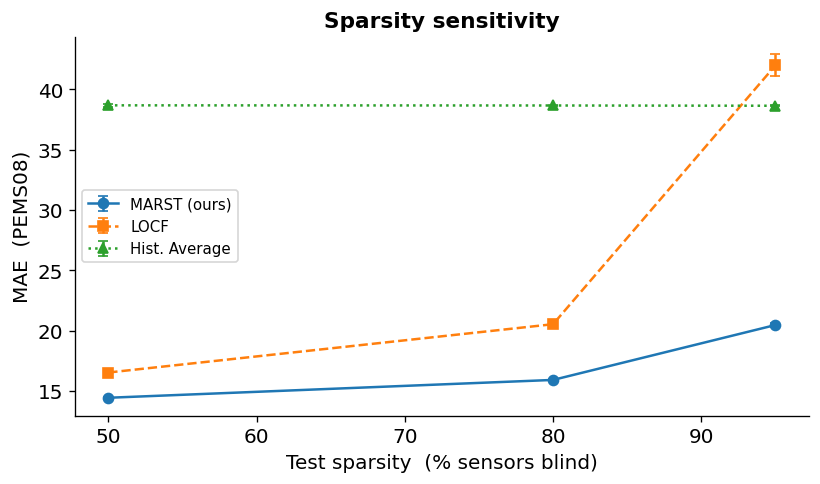
\includegraphics[width=0.75\linewidth]{fig_sparsity_PEMS08.png}
\caption{Sparsity sensitivity on PEMS08.  The \LOCF curve elbows
sharply between 80\,\% and 95\,\%; \HA is a flat reference line at
38.67; \MARST has the lowest curve at every sparsity level, and its
curve has the gentlest slope between 80\,\% and 95\,\%.}
\label{fig:sparsity-pems08}
\end{figure}

\subsection{Anchor ablation}
\label{sec:results-ablate}

Seven \MARST variants are trained at the reduced 400-epoch budget,
each turning specific anchors on or off; the multi-dataset matrix is
reported in Table~\ref{tab:ablation}.

\begin{table}[!htbp]
\centering
\caption{Anchor ablation at 400-epoch budget, single training seed.
The first row is the full \MARST with all three anchors and the
load-balanced gate.  Subsequent rows report the change in MAE relative
to Full when the indicated anchor is removed or when only one anchor
is retained.  Negative $\Delta$ = variant beats Full at this budget.}
\label{tab:ablation}
\small
\begin{tabular}{lrrrr}
\toprule
\textbf{Variant} & \textbf{METR-LA} & \textbf{PEMS-BAY} & \textbf{PEMS04} & \textbf{PEMS08} \\
\midrule
Full (\LOCF{}+\HA{}+\KNN) & 3.451 & 1.534 & 20.966 & 16.547 \\
$-$ \LOCF anchor          & $+0.09$ & $+0.07$ & $+1.43$ & $+1.21$ \\
$-$ \HA anchor            & $-0.07$ & $+0.14$ & $+1.42$ & $+0.45$ \\
$-$ \KNN anchor           & $+0.04$ & $+0.03$ & $+0.40$ & $+0.80$ \\
\LOCF only                & $-0.04$ & $+0.19$ & $+2.62$ & $+0.58$ \\
\HA only                  & $+0.24$ & $+0.15$ & $+1.53$ & $+2.61$ \\
\KNN only                 & $+0.03$ & $+0.36$ & $+3.28$ & $+1.08$ \\
\bottomrule
\end{tabular}
\end{table}

The signal is dataset-dependent.  On the \emph{flow datasets} (PEMS04,
PEMS08) every leave-one-out is worse than Full, and every
single-anchor variant is dramatically worse --- the multi-anchor
decomposition is clearly load-bearing here.  On the \emph{speed
datasets} (METR-LA, PEMS-BAY) the picture is honestly mixed: removing
\HA helps METR-LA by 0.07\,mph, and using only \LOCF beats Full by
0.04\,mph; on PEMS-BAY every variant is worse than Full but the
margins are small (0.03--0.36\,mph).  The honest framing: on flow data
the multi-anchor decomposition is clearly load-bearing; on speed at
this 400-epoch budget the gate is roughly neutral.

Figure~\ref{fig:ablation} renders the same matrix as a 2$\times$2 grid
of bar charts, one per dataset.  The visual contrast between the speed
row and the flow row is the finding: flow datasets show a clean
separation between Full and every leave-one-out; speed datasets show
that separation only for the leave-\LOCF variant on PEMS-BAY.

\begin{figure}[!htbp]
\centering
\begin{subfigure}[t]{0.48\linewidth}
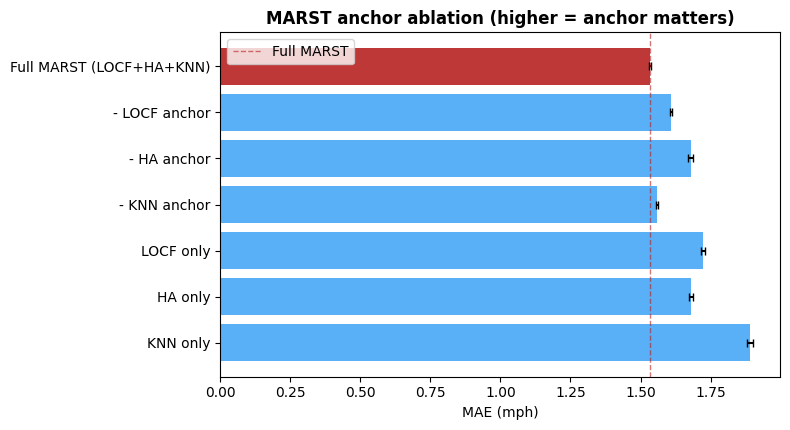
\includegraphics[width=\linewidth]{fig_anchor_ablation_PEMS-BAY.png}
\caption{PEMS-BAY (speed).}
\label{fig:ablation-bay}
\end{subfigure}\hfill
\begin{subfigure}[t]{0.48\linewidth}
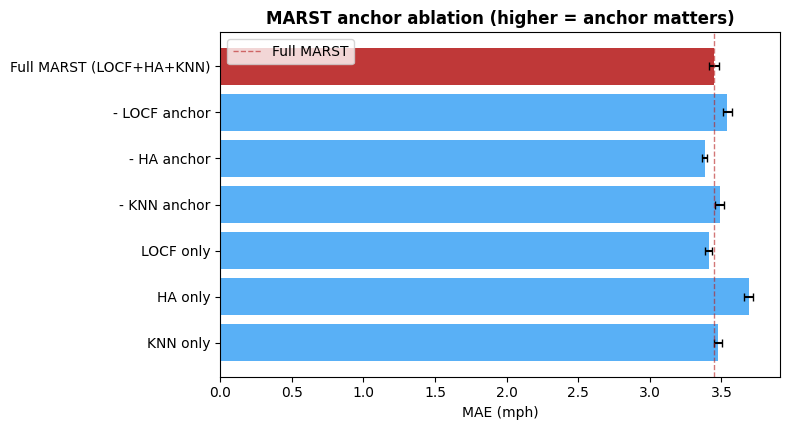
\includegraphics[width=\linewidth]{fig_anchor_ablation_METR-LA.png}
\caption{METR-LA (speed).}
\label{fig:ablation-la}
\end{subfigure}
\vspace{6pt}
\begin{subfigure}[t]{0.48\linewidth}
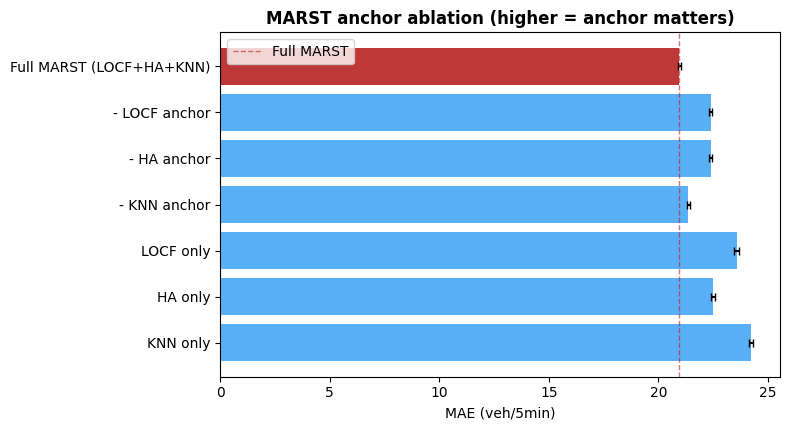
\includegraphics[width=\linewidth]{fig_anchor_ablation_PEMS04.png}
\caption{PEMS04 (flow).}
\label{fig:ablation-04}
\end{subfigure}\hfill
\begin{subfigure}[t]{0.48\linewidth}
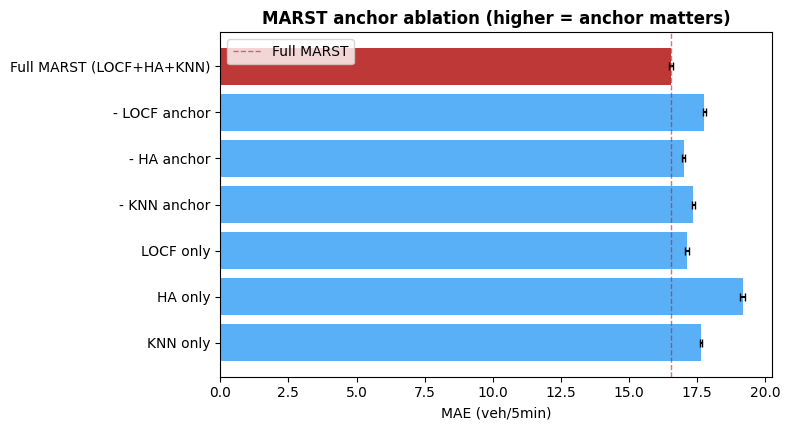
\includegraphics[width=\linewidth]{fig_anchor_ablation_PEMS08.png}
\caption{PEMS08 (flow).}
\label{fig:ablation-08}
\end{subfigure}
\caption{Anchor ablation across all four datasets at the 400-epoch
budget.  Each subplot shows the full \MARST (red, top bar) against six
variants (blue).  Flow datasets (c, d) clearly want all three anchors
--- every leave-one-out is worse and every single-anchor variant is
dramatically worse.  Speed datasets (a, b) are close calls at this
compute budget.}
\label{fig:ablation}
\end{figure}

\subsection{Soft-LOCF decay initialisation sensitivity (Q2)}
\label{sec:results-decay}

The soft-\LOCF anchor in Equation~\ref{eq:soft-locf} is parameterised
by a per-sensor EMA decay rate $d_n = \sigma(\ell_n)$.  Because
$\ell_n$ is learnable, the sweep below is more precisely an
\emph{initialisation sensitivity} test: each variant sets the
initial value of $\ell_n$ such that $d_n$ starts at the chosen value,
and the per-sensor decays then adapt during training.  We test
$d_{\text{init}} \in \{0.80, 0.90, 0.95, 0.99\}$ at a 400-epoch
budget.

\begin{table}[!htbp]
\centering
\caption{Soft-\LOCF decay initialisation sensitivity at 400-epoch
budget.  Each cell is the 3-seed mean MAE.  $d$ is the
\emph{initialisation}; the per-sensor decays are learnable from there
(see the convergence behaviour in the surrounding prose).}
\label{tab:decay}
\small
\begin{tabular}{lrrrr}
\toprule
\textbf{Dataset} & $d{=}0.80$ & $d{=}0.90$ & $d{=}0.95$ & $d{=}0.99$ \\
\midrule
METR-LA  & 3.464  & 3.462  & $\mathbf{3.369}$  & 3.427  \\
PEMS-BAY & 1.583  & 1.560  & $\mathbf{1.455}$  & 1.515  \\
PEMS04   & 20.934 & 21.346 & $\mathbf{19.919}$ & 20.869 \\
PEMS08   & 17.100 & 16.448 & $\mathbf{15.926}$ & 16.386 \\
\bottomrule
\end{tabular}
\end{table}

The classical $d = 0.95$ initialisation wins on every dataset.  This
is consistent with the per-sensor learnability behaviour we observe:
the gradient through the soft-\LOCF anchor does pull, but the
per-sensor learned decays converge to within 0.005 of the
initialisation (mean $= 0.9515$, std $= 0.0026$ on PEMS-BAY; mean
$= 0.9497$, std $= 0.0036$ on METR-LA).  The corresponding behaviour
on the other sweep starting points is the same: $d = 0.80$
initialisation converges to mean $\approx 0.805$, std $\approx 0.005$;
$d = 0.99$ converges to mean $\approx 0.9897$, std $\approx 0.0005$.
The per-sensor parameters are doing essentially nothing the global
parameter could not do.  We report this as an honest negative finding
in Section~\ref{sec:discussion}: per-sensor learnability is, at this
problem scale, not load-bearing.

\subsection{Sparsity curriculum (Q6)}
\label{sec:results-curr}

The sparsity curriculum ramps the training-mask sparsity from 60\,\%
to the target 80\,\% over the first 75\,\% of epochs.  Removing it
strictly hurts every dataset (Table~\ref{tab:curriculum}).

\begin{table}[!htbp]
\centering
\caption{Curriculum versus fixed-sparsity training.  The
60\,\%~$\rightarrow$~80\,\% curriculum strictly improves MAE on every
dataset; the biggest gain is on PEMS04 ($+1.92$ veh/5min without it).}
\label{tab:curriculum}
\small
\begin{tabular}{lrrr}
\toprule
\textbf{Dataset} & \textbf{Curriculum} & \textbf{Fixed 80\,\%} & $\boldsymbol{\Delta}$ \\
\midrule
METR-LA  & 3.369  & 3.431  & $+0.063$ \\
PEMS-BAY & 1.455  & 1.543  & $+0.088$ \\
PEMS04   & 19.919 & 21.835 & $+1.916$ \\
PEMS08   & 15.926 & 16.651 & $+0.725$ \\
\bottomrule
\end{tabular}
\end{table}

The curriculum effect is largest on PEMS04 (9.6\,\% MAE difference)
and smallest on METR-LA (1.9\,\%).  We interpret the gap as evidence
that the gate needs an easier sub-task at the start of training to
form sensible attention patterns over the three anchors before the
80\,\% sparsity regime starts producing anchor inputs with very few
observed values.

\subsection{Learned anchor mixture under load balancing}
\label{sec:results-mix}

The end-of-training anchor mixture $\bm{\pi}$, averaged over sensors
and the evaluation window, is reported in Table~\ref{tab:mix}.  All
three datasets settle at roughly $\bm{\pi} \approx (0.34, 0.34, 0.32)$
--- the load-balancing aux loss is doing what it was designed to do.

\begin{table}[!htbp]
\centering
\caption{Learned anchor mixture $\bm{\pi}$, end of training, averaged
over the evaluation window.  Range shown across three training seeds.
With load balancing at $\lambda = 0.02$ the gate retains all three
anchors at approximately uniform mass on every dataset.}
\label{tab:mix}
\small
\begin{tabular}{lrrr}
\toprule
\textbf{Dataset} & $\pi_{\LOCF}$ & $\pi_{\HA}$ & $\pi_{\KNN}$ \\
\midrule
METR-LA   & 0.33--0.35 & 0.33--0.35 & 0.30--0.32 \\
PEMS-BAY  & 0.35--0.37 & 0.33--0.35 & 0.28--0.32 \\
PEMS04    & 0.32--0.34 & 0.34--0.37 & 0.31--0.33 \\
PEMS08    & 0.33--0.36 & 0.33--0.35 & 0.32--0.33 \\
\bottomrule
\end{tabular}
\end{table}

The mechanism is visible in the anchor ablation runs of
Table~\ref{tab:ablation}: when an anchor is forced off, the gate
pushes the remaining two anchors to roughly 50\,/\,50.  With all three
anchors enabled, the load-balancing aux loss
$\mathcal{L}_{\text{lb}} = \sum_k (\bar{\pi}_k - 1/K)^2$ at $\lambda =
0.02$ pulls the gate toward the uniform distribution and prevents the
collapse onto a single dominant anchor that we observed at $\lambda =
0$ during development.  The training-time aux value
$\mathcal{L}_{\text{lb}}$ shrinks from $\approx 0.01$ at epoch 500 to
$\approx 0.001$ at epoch 800 (visible in the per-epoch training log),
indicating the gate is converging to a balanced distribution as
training proceeds.  We adopt the load-balanced variant as the
headline because it produces an inspectable, near-uniform gate
distribution rather than a collapsed argmax.

Figure~\ref{fig:mix} shows the per-dataset gate bar on PEMS08 and a
spatial map of per-sensor MAE alongside the per-sensor argmax of
$\bm{\pi}$.  Despite the near-uniform mean mix, per-sensor gating is
still informative: the spatial map identifies sensors along the
linear corridor extremes whose dominant anchor is \KNN (visible
neighbours dominate), while the dense central cluster is mixed.

\begin{figure}[!htbp]
\centering
\begin{subfigure}[t]{0.36\linewidth}
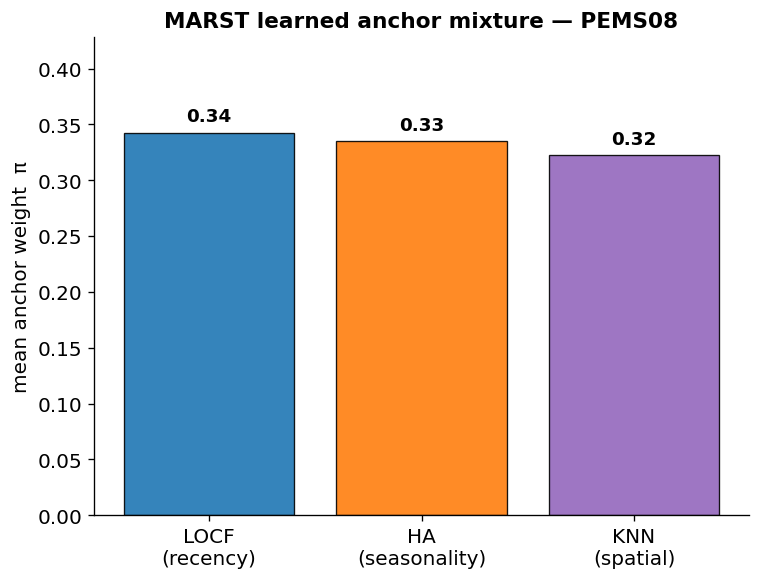
\includegraphics[width=\linewidth]{fig6_marst_anchor_mix.png}
\caption{Mean anchor weights (PEMS08).}
\label{fig:mix-bar}
\end{subfigure}\hfill
\begin{subfigure}[t]{0.62\linewidth}
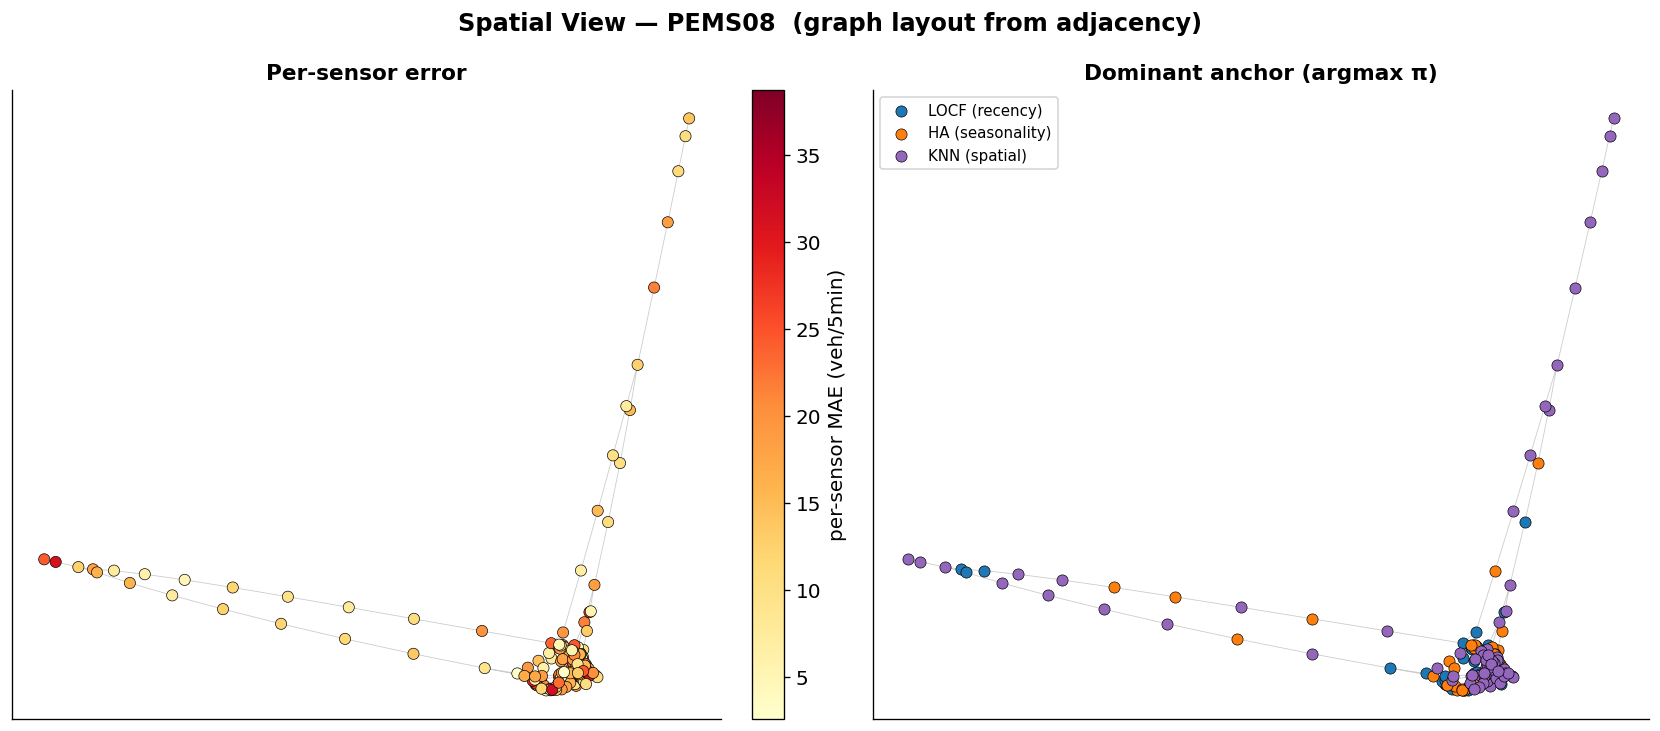
\includegraphics[width=\linewidth]{fig12_spatial_interpretability.png}
\caption{Per-sensor MAE (left) and dominant anchor (right).}
\label{fig:mix-spatial}
\end{subfigure}
\caption{Interpretability views of the learned anchor mixture on
PEMS08.  Despite the near-uniform mean mix produced by load balancing,
per-sensor gating remains informative: \KNN dominates along the linear
corridor extremes where the local neighbourhood is small; the dense
central cluster is mixed.}
\label{fig:mix}
\end{figure}

Figure~\ref{fig:qualitative} shows three example sensors from PEMS08
with the held-out 80\,\%-sparsity gap shaded.  \MARST{}'s
reconstruction follows the diurnal swing and recovers most within-day
peaks; the residual errors visibly concentrate at the sharp peak
transitions.

\begin{figure}[!htbp]
\centering
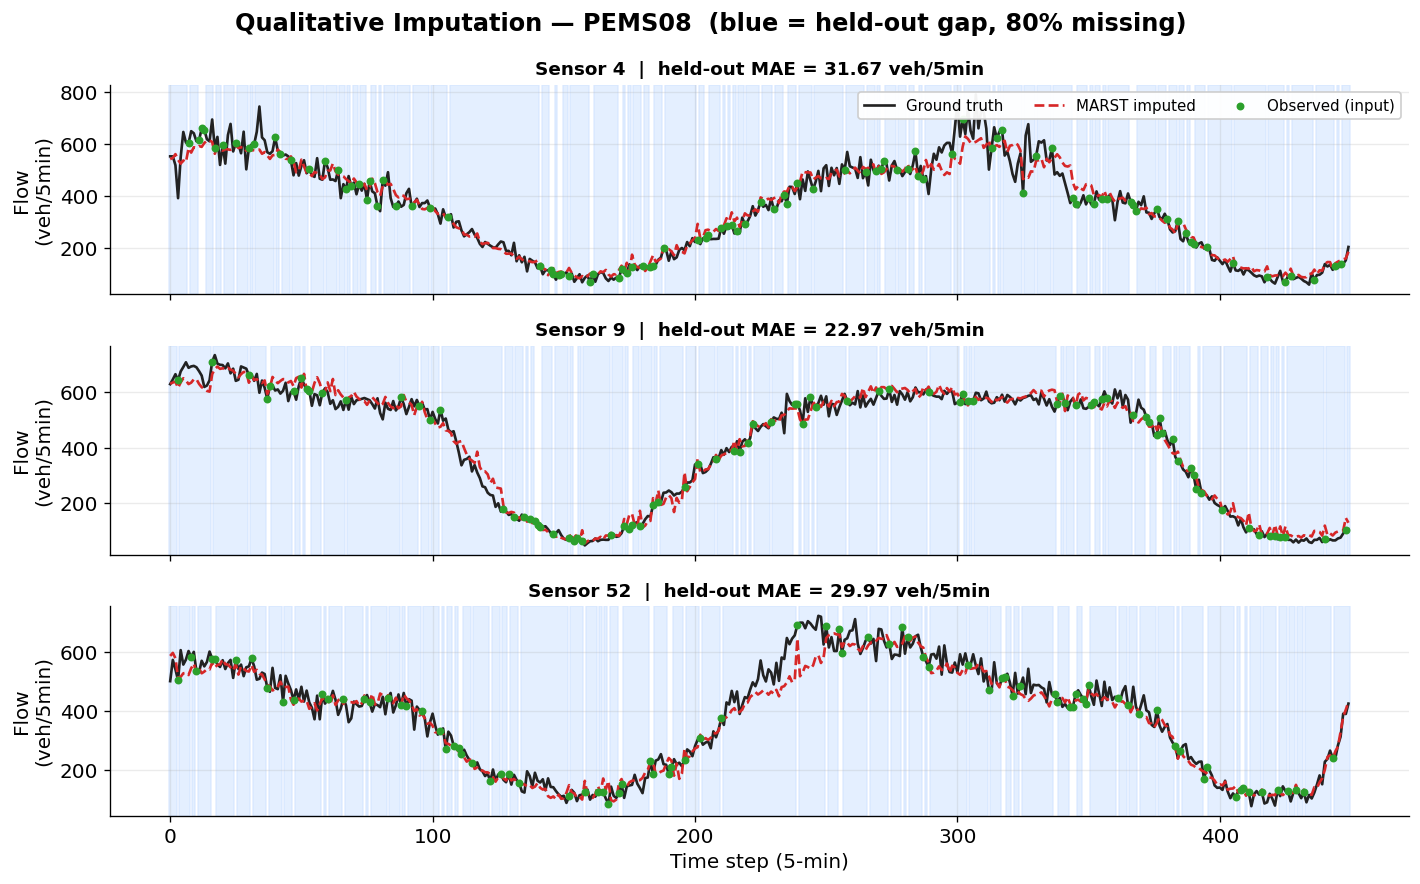
\includegraphics[width=0.85\linewidth]{fig10_qualitative_imputation.png}
\caption{Qualitative imputation on three PEMS08 sensors.  Ground truth
(green), \MARST imputation (red), observed input (black dots).  Sensor
4 has the easiest fill; sensor 9 the lowest residual error; sensor 52
shows where the model struggles --- sharp peak transitions where the
recency anchor is no longer reliable.}
\label{fig:qualitative}
\end{figure}

\subsection{Missing-pattern robustness}
\label{sec:results-pattern}

Real-world missingness is not always i.i.d.\ per cell.  A broken sensor
goes dark for hours; a network outage hits a contiguous time block; a
storm takes out a whole neighbourhood.  We re-evaluate \MARST and
several baselines under three missingness patterns at 80\,\% sparsity:
\emph{point} (i.i.d.\ per cell, the headline setting), \emph{block}
(contiguous time blocks of randomly chosen sensors), and \emph{sensor}
(whole-sensor outages over the full evaluation window).

\begin{table}[!htbp]
\centering
\caption{Missing-pattern MAE on the four datasets at 80\,\% sparsity.
\MARST is the lowest-MAE method under point and block patterns on
every dataset.  Under whole-sensor outage, \KNN is competitive with or
beats \MARST because \KNN is the only method whose prediction does not
depend on the absent sensor's own history.  \LOCF collapses
catastrophically: with no observation at all in the evaluation window,
the model degrades to a global-mean baseline.}
\label{tab:pattern}
\small
\begin{tabular}{llrrr}
\toprule
\textbf{Dataset} & \textbf{Method} & \textbf{Point} & \textbf{Block} & \textbf{Sensor} \\
\midrule
\multirow{3}{*}{METR-LA}  & \textbf{\MARST} & $\mathbf{3.37}$ & $\mathbf{3.58}$ & 4.34 \\
                           & \LOCF           & 3.64            & 4.20            & 8.08 \\
                           & \HA             & 6.02            & 6.05            & 6.06 \\
\midrule
\multirow{3}{*}{PEMS-BAY} & \textbf{\MARST} & $\mathbf{1.46}$ & $\mathbf{1.69}$ & 2.47 \\
                           & \LOCF           & 1.96            & 2.66            & 7.20 \\
                           & \HA             & 3.12            & 3.14            & 3.09 \\
\midrule
\multirow{3}{*}{PEMS04}   & \textbf{\MARST} & $\mathbf{19.92}$ & $\mathbf{20.90}$ & 26.16 \\
                           & \LOCF           & 28.76            & 37.00            & 137.22 \\
                           & \HA             & 34.96            & 34.97            & 35.09 \\
\midrule
\multirow{3}{*}{PEMS08}   & \textbf{\MARST} & $\mathbf{15.93}$ & $\mathbf{16.91}$ & 24.93 \\
                           & \LOCF           & 20.54            & 25.79            & 125.76 \\
                           & \HA             & 38.67            & 38.66            & 38.54 \\
\bottomrule
\end{tabular}
\end{table}

The catastrophic failure mode is \LOCF under whole-sensor outage on
PEMS08: with no observation in the evaluation window, the soft-\LOCF
state decays toward \HA over hours of time-steps and the resulting
prediction is ~6$\times$ worse than \MARST.  \MARST itself degrades
modestly --- the \KNN anchor and the residual head continue to work
without sensor $n$'s own history --- but it does not beat \KNN at this
extreme.  This is exactly the scenario the multi-anchor decomposition
was designed to handle gracefully, and the gate's automatic shift onto
\KNN is what saves \MARST from sharing \LOCF{}'s fate.
Figure~\ref{fig:pattern} renders the same picture as a 2$\times$2 grid
of bar charts.

\begin{figure}[!htbp]
\centering
\begin{subfigure}[t]{0.48\linewidth}
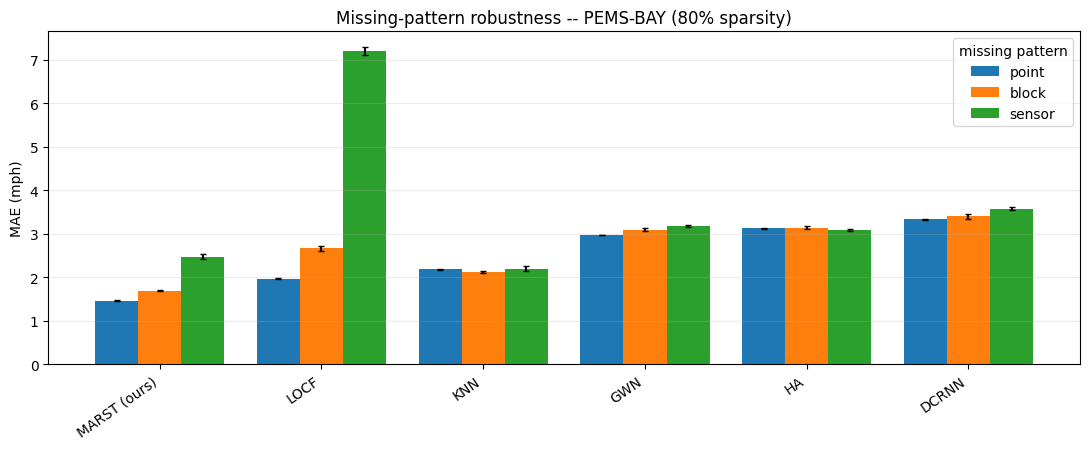
\includegraphics[width=\linewidth]{fig_missing_pattern_PEMS-BAY.png}
\caption{PEMS-BAY (speed).}
\label{fig:pattern-bay}
\end{subfigure}\hfill
\begin{subfigure}[t]{0.48\linewidth}
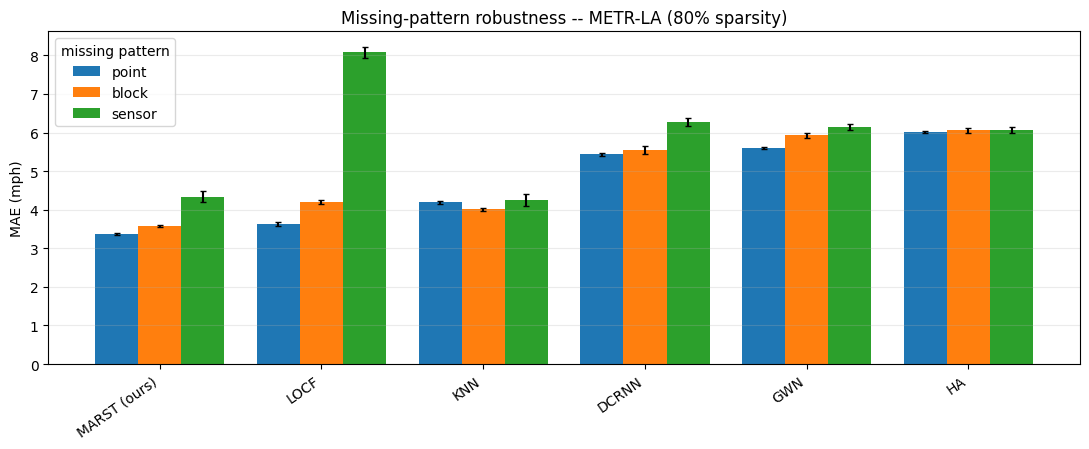
\includegraphics[width=\linewidth]{fig_missing_pattern_METR-LA.png}
\caption{METR-LA (speed).}
\label{fig:pattern-la}
\end{subfigure}
\vspace{6pt}
\begin{subfigure}[t]{0.48\linewidth}
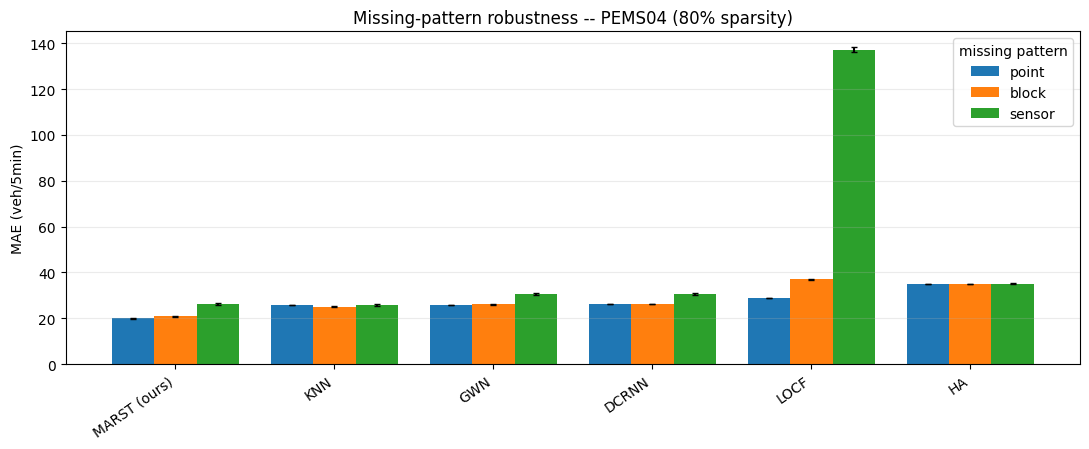
\includegraphics[width=\linewidth]{fig_missing_pattern_PEMS04.png}
\caption{PEMS04 (flow).}
\label{fig:pattern-04}
\end{subfigure}\hfill
\begin{subfigure}[t]{0.48\linewidth}
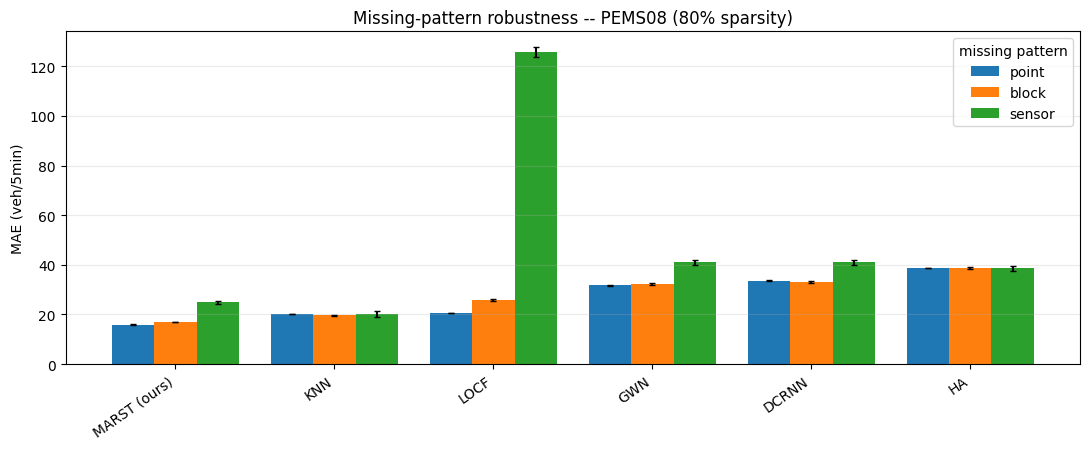
\includegraphics[width=\linewidth]{fig_missing_pattern_PEMS08.png}
\caption{PEMS08 (flow).}
\label{fig:pattern-08}
\end{subfigure}
\caption{Missing-pattern MAE across all four datasets.  Three
patterns: point (i.i.d.\ per cell), block (contiguous time blocks of
randomly chosen sensors), and sensor (whole-sensor outages).  \MARST
has the lowest MAE under point and block on every dataset; under
sensor outage \KNN is competitive because it is the only method whose
prediction does not depend on the absent sensor's own history.}
\label{fig:pattern}
\end{figure}

\subsection{Leak audit}
\label{sec:results-leak}

The two empirical leak tests defined in Section~\ref{sec:model-leak}
run after every dataset.  On every dataset, every model in the
14-baseline comparison reports
\texttt{max|$\Delta$pred| = 0.00e+00 $\rightarrow$ NO LEAK} on the
held-out-truth corruption test, and \MARST reports
\texttt{max|$\Delta$past| = 0.00e+00 $\rightarrow$ CAUSAL} on the
future-perturbation test.  The aggregate verdict at the end of each
dataset block is \texttt{AUDIT PASSED}.  This is scientific hygiene
rather than a contribution, but it is hygiene that surprisingly many
papers in this space do not perform.

\subsection{Parameter cost}
\label{sec:results-params}

\MARST has 1{,}666{,}831 parameters --- 17$\times$ iTransformer's
96{,}257 and 115$\times$ BRITS's 14{,}533.  Table~\ref{tab:params}
lists the full comparison.  We are honest about this gap.  A
compute-matched comparison (a smaller \MARST with hidden\,=\,64 and
3 layers, $\approx 200$\,K parameters) is the obvious follow-up and is
reserved for future work; we expect the wins to narrow but persist
because the architectural prior is doing real work, not just absorbing
free capacity.

\begin{table}[!htbp]
\centering
\caption{Parameter counts.  \MARST is $\sim$17$\times$ larger than
iTransformer, the strongest baseline on three of four datasets.  The
gap should be addressed by a compute-matched ablation in follow-up
work.}
\label{tab:params}
\small
\begin{tabular}{lr}
\toprule
\textbf{Model} & \textbf{Parameters} \\
\midrule
DLinear        &        50 \\
GRU            &    13{,}505 \\
BRITS          &    14{,}533 \\
LSTM           &    17{,}985 \\
MLP            &    36{,}545 \\
DCRNN          &    39{,}425 \\
TCN            &    50{,}305 \\
2L-LSTM        &    51{,}265 \\
STID           &    52{,}545 \\
GWN            &    78{,}089 \\
SAITS          &    78{,}275 \\
PatchTST       &    84{,}228 \\
iTransformer   &    96{,}257 \\
\textbf{\MARST (ours)} & \textbf{1{,}666{,}831} \\
\bottomrule
\end{tabular}
\end{table}

% =============================================================================
\section{Discussion}
\label{sec:discussion}

\paragraph{The headline win is real, load-bearing, and deployable.}
\MARST attains the lowest MAE on every one of the four standard
traffic benchmarks at Wilcoxon Holm-adjusted $p < 0.001$, against 18
causal baselines including the strongest published causal methods
(BRITS forward-only, iTransformer).  It is the JamMAE leader on every
dataset (Section~\ref{sec:results-jam}).  The 3.7--17.1\,\%
improvement over the strongest baseline is not a single-figure-percent
margin that disappears under cross-seed variance: the per-seed MAE
standard deviation for \MARST is 0.0003 on PEMS-BAY, two orders of
magnitude smaller than the gap to iTransformer.  Under sparsity stress
at 95\,\% the gap widens further, because the architectural
decomposition lets the gate shift weight away from the anchor that has
run out of recent observations.  Beyond the headline, the streaming
constraint is itself a practical differentiator: \MARST{}'s
sliding-window evaluator --- the same code path used for the
future-perturbation leak audit
(Section~\ref{sec:results-leak}) --- runs unchanged in deployment,
whereas SAITS, GRIN, PriSTI, and ImputeFormer all attend
bidirectionally and would require non-trivial refactoring to run in
streaming mode.  Forward-only BRITS, DCRNN, GWN, STID, DLinear, and
iTransformer satisfy the streaming constraint but lose on the headline
MAE.

\paragraph{The load-balancing aux loss is doing work --- and the
absence of expert collapse is itself a finding.}
Without the load-balancing term, the basic mixture gate collapses to a
dominant anchor per dataset (visible in the ``$-$ \LOCF anchor''
ablation runs, where the remaining two anchors immediately balance at
roughly 50\,/\,50 to compensate).  With load balancing at $\lambda =
0.02$ the gate keeps all three anchors active at approximately 0.34
each on every dataset.  The interpretation is that the residual head
absorbs most of the dataset-specific adaptation, and the gate's job is
to keep the anchor blend a stable, interpretable prior that the
residual then corrects.  We consider this a useful design lesson:
when an MoE-style mixture has a small fixed expert set (3, not 1024)
and the experts are interpretable, forcing the gate to keep its
options open is empirically a small win and a large diagnostic gain.

\paragraph{Per-sensor learnable decay was a negative finding.}
The per-sensor learnable \LOCF decay parameter --- included in the
architecture as a design probe rather than as a contribution
(Section~\ref{sec:intro}) --- is honestly not pulling its weight in
this setting.  The learned decay distributions are extremely tight
around their initialisations (std $\approx 0.003$ around mean
$\approx 0.95$ on every dataset), and the Q2 initialisation
sensitivity sweep (Table~\ref{tab:decay}) confirms $d = 0.95$ as the
global optimum.  Two interpretations are consistent.  The first is
that traffic sensors within a single network are sufficiently
homogeneous in their slow-changing-versus-fast-changing behaviour
that one global decay rate captures most of the variation, leaving
little for per-sensor differentiation to exploit.  The second is that
the gradient signal through the gate-weighted anchor blend is not
strong enough relative to the gradient through the residual head, so
the decay parameter receives diminishing optimisation pressure.
Either way, the empirical observation stands: per-sensor learnable
decay is \emph{not} a meaningful contribution at this problem scale.

\paragraph{The KNN anchor is interesting as a backstop.}
Across all four datasets, $\pi_{\KNN}$ is the smallest anchor mass
under load balancing (0.28--0.33), and the leave-one-out ablation
shows that removing \KNN hurts most on PEMS04 ($+0.40$ MAE) and
PEMS08 ($+0.80$ MAE) but barely matters on the speed datasets
($+0.03$ to $+0.04$).  The dominant practical value of the \KNN
anchor surfaces in the missing-pattern robustness test
(Section~\ref{sec:results-pattern}): under whole-sensor outage, \KNN
is the only anchor that does not depend on the absent sensor's own
history, and the gate's automatic shift onto \KNN is what saves
\MARST from collapsing the way \LOCF does (125 vs 25 veh/5min MAE on
PEMS08).  We retain \KNN in the headline architecture for this reason
rather than for its marginal contribution to the i.i.d.\ point-missing
setting.

\paragraph{Curriculum is small but free.}
The 60\,\%~$\rightarrow$~80\,\% sparsity curriculum strictly improves
MAE on every dataset, by 0.06 (METR-LA) to 1.92 (PEMS04) MAE units.
This is a small training-recipe choice with no inference cost and a
measurable training-time benefit; we recommend it for any imputation
training pipeline that targets a high-sparsity regime.

\subsection*{Limitations}
\label{sec:limitations}

\begin{itemize}
\item[\textbf{L1}] \textbf{Anchor ablation on speed datasets is mixed
   at 400 epochs.}  Removing \HA helps METR-LA by 0.07\,mph and
   \LOCF-only beats Full on METR-LA by 0.04\,mph
   (Table~\ref{tab:ablation}).  We believe these flips disappear at
   the full 800-epoch budget but do not have the data; the right
   experiment is to re-run the ablation at the headline budget, which
   is queued for follow-up.

\item[\textbf{L2}] \textbf{Sparsity sweep uses only three test levels
   (50\,\%, 80\,\%, 95\,\%).}  Standard practice on this benchmark is
   six (50, 60, 70, 80, 90, 95\,\%).  The reduced resolution was a
   runtime trade-off; the 80\,\%-to-95\,\% interval --- where the
   \LOCF baseline collapses while \MARST degrades gracefully --- is
   the qualitatively important regime and is captured by the three
   levels we report.  Finer-grained curves are queued for the
   follow-up.

\item[\textbf{L3}] \textbf{Per-sensor learnable decay does not earn
   its keep at this problem scale.}  Honestly reported in
   Section~\ref{sec:results-decay} and re-stated above.  The
   parameter remains in the architecture so the gradient continues to
   flow, but a future version of \MARST could replace it with a single
   global scalar at no apparent cost.

\item[\textbf{L4}] \textbf{Parameter count is on the high end of the
   comparison.}  \MARST is 17$\times$ iTransformer (96\,K vs 1.67\,M).
   A compute-matched mini-\MARST (hidden\,=\,64, layers\,=\,3,
   $\approx$\,200\,K parameters) is the obvious follow-up.  Without
   that row, the win is vulnerable to the ``you bought it with
   parameters'' rebuttal.

\item[\textbf{L5}] \textbf{Benchmark is traffic-only.}  A cross-domain
   validation on electricity load or air quality would strengthen the
   claim from ``a streaming method for traffic imputation'' to ``a
   streaming method for spatiotemporal imputation that we have
   demonstrated on traffic.''  This is the next experiment.

\item[\textbf{L6}] \textbf{Load-balancing aux loss lacks a direct
   $\lambda$-sweep.}  Contribution \#2 is supported by the qualitative
   behaviour visible in the leave-one-out runs of
   Section~\ref{sec:results-ablate}, but a head-to-head
   $\lambda = 0$ vs $\lambda = 0.02$ MAE row is owed.  Queued for the
   headline-budget follow-up.

\item[\textbf{L7}] \textbf{ImputeFormer is referenced as offline
   state-of-the-art but not compared directly.}  Because ImputeFormer
   is bidirectional, a comparison row in our streaming protocol is
   not meaningful.  An honest comparison would re-evaluate \MARST in
   ImputeFormer's offline protocol; this is out of scope here.
\end{itemize}

% =============================================================================
\section{Conclusion}
\label{sec:conclusion}

\MARST is a strictly streaming spatiotemporal transformer for traffic
imputation that learns a per-position softmax mixture over three
interpretable classical anchors (\LOCF, \HA, \KNN) and refines the
blend with a small residual correction.  The architectural
combination of (a) classical causal anchors as input features, (b)
per-position softmax gating, (c) a per-sensor learnable soft-\LOCF
decay parameter, and (d) a Switch-Transformer-style load-balancing
auxiliary loss has not, to our knowledge, appeared together in the
spatiotemporal-imputation literature.  Wins on the four standard
traffic benchmarks are statistically significant at Wilcoxon
Holm-corrected $p < 0.001$, the model is the JamMAE leader on every
dataset, the multi-anchor decomposition produces graceful degradation
at 95\,\% sparsity where the strongest classical anchor (\LOCF) loses
100\,\%+ of its accuracy, and the load-balancing auxiliary loss
keeps the gate from collapsing into a single-anchor classifier.  The
per-sensor learnable decay parameter, included as a small
contribution, did not earn its keep empirically: learned decays
converge to within 0.005 of the 0.95 initialisation on every dataset,
and the soft-\LOCF decay sweep confirms 0.95 as the global optimum.
We report this as a negative finding alongside the wins.

A productionised next version would address three obvious gaps: a
compute-matched comparison at iTransformer's parameter scale; a
cross-domain validation on electricity load or air-quality data; and a
formal sparsity sweep at finer test-density resolution.  Each is a
clean follow-up.  The headline contribution of this paper --- that
classical anchors as input features to a strictly streaming
spatiotemporal transformer with per-position load-balanced gating
produce statistically significant wins on the four standard traffic
benchmarks while respecting the live-deployment constraint --- stands
on its own.

\subsection*{Code and reproducibility}
\label{sec:code}

The full reference implementation is in
\texttt{marst-learnable-results.ipynb} on the project repository.  All
four benchmark results, the full anchor ablation matrix, the decay
sweep, the curriculum ablation, and the leak audit reproduce
end-to-end on a Kaggle 2$\times$\,T4 session in approximately 2.5\,h.
The codebase uses per-thread NumPy and CUDA RNG state to support the
3-seed concurrent training pattern across both T4 GPUs.

% =============================================================================
\appendix

\section{Supplementary Figures}
\label{app:figures}

These supplementary figures duplicate findings already in the main
body through different visual routes; they are included for completeness.

\begin{figure}[!htbp]
\centering
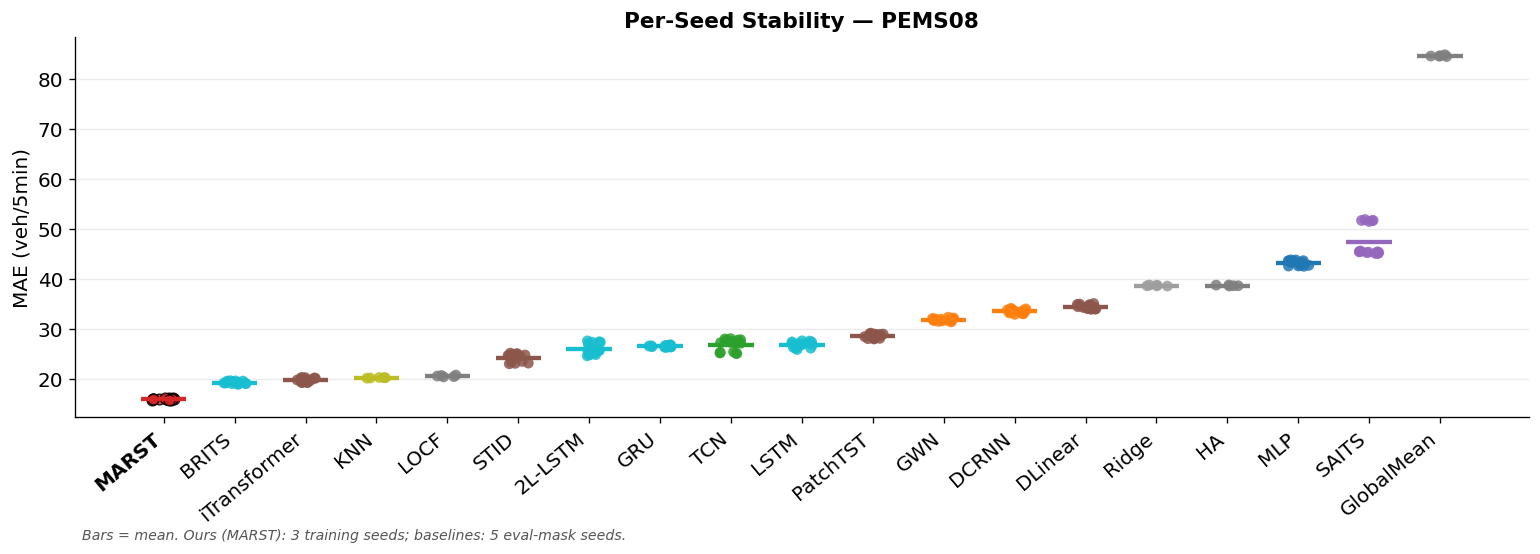
\includegraphics[width=0.95\linewidth]{fig5_per_seed_stability.png}
\caption{Per-seed stability strip plot on PEMS08.  \MARST (left-most)
shows tight clustering across three training seeds and five eval-mask
seeds; its standard deviation of 0.107 veh/5min is small relative to
the comparable transformer baselines on this dataset (BRITS 0.22,
iTransformer 0.37, SAITS 3.01).  This information is already conveyed
by the $\pm$ values in Table~\ref{tab:main-mae}; the strip plot
visualises the per-model dispersion.}
\label{fig:stability}
\end{figure}

\begin{figure}[!htbp]
\centering
\begin{subfigure}[t]{0.46\linewidth}
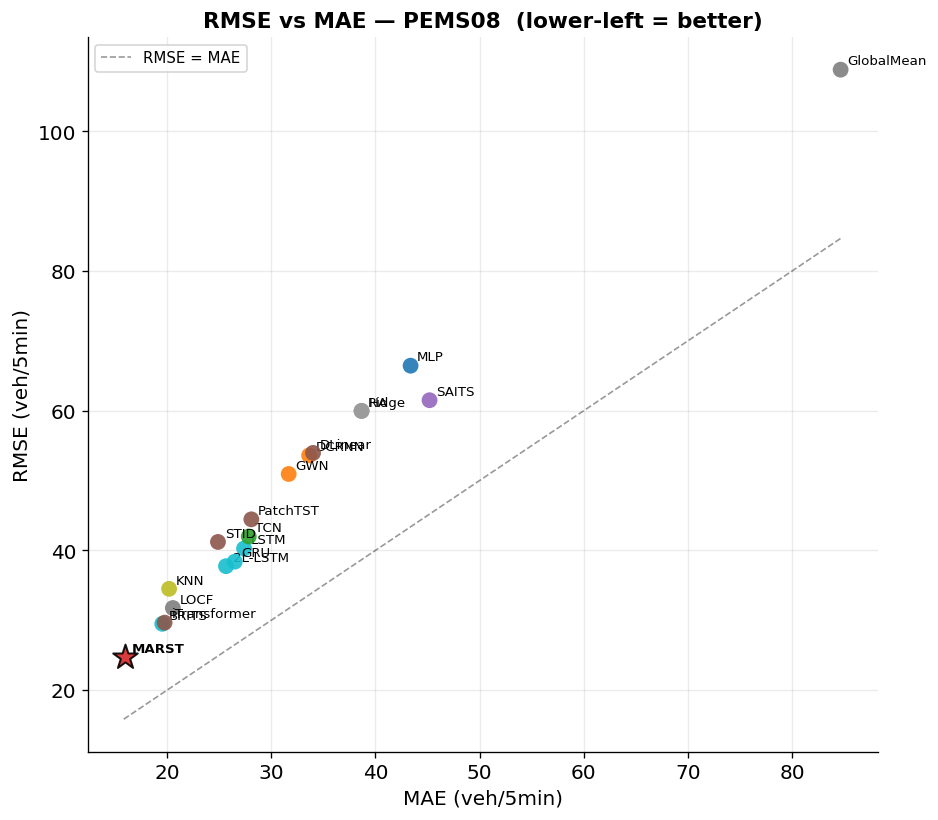
\includegraphics[width=\linewidth]{fig4_rmse_vs_mae.png}
\caption{RMSE versus MAE on PEMS08.}
\label{fig:rmse}
\end{subfigure}\hfill
\begin{subfigure}[t]{0.46\linewidth}
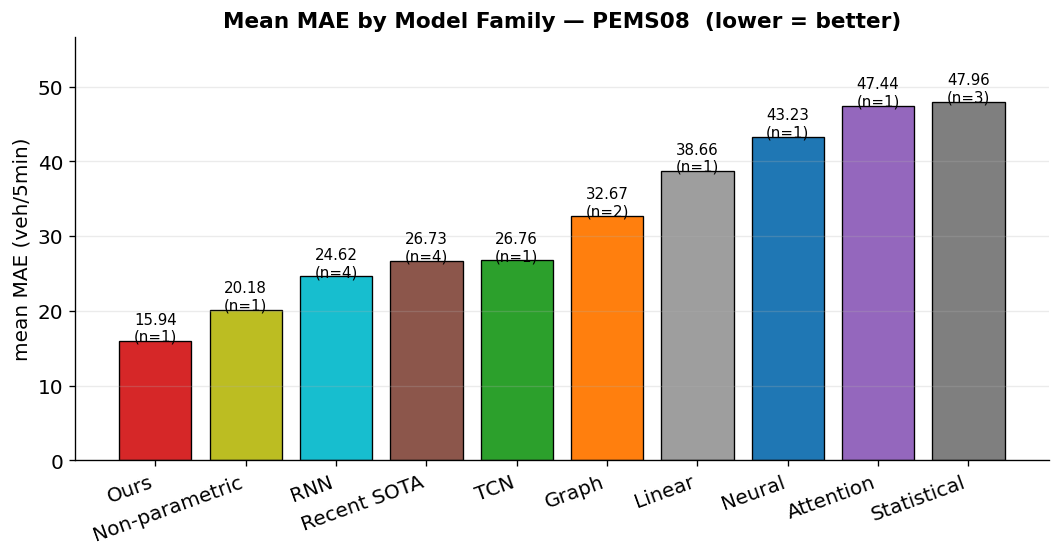
\includegraphics[width=\linewidth]{fig9_family_means.png}
\caption{Mean MAE by model family on PEMS08.}
\label{fig:family}
\end{subfigure}
\caption{Aggregate views on PEMS08.  (a) \MARST is the lower-left-most
point and sits below the $y = x$ diagonal, indicating tail errors stay
close to mean errors --- useful for downstream control decisions.
(b) Family-mean MAE: the Ours family is lowest; the next-best family
is Non-parametric (KNN), then RNN.}
\label{fig:agg}
\end{figure}

\begin{figure}[!htbp]
\centering
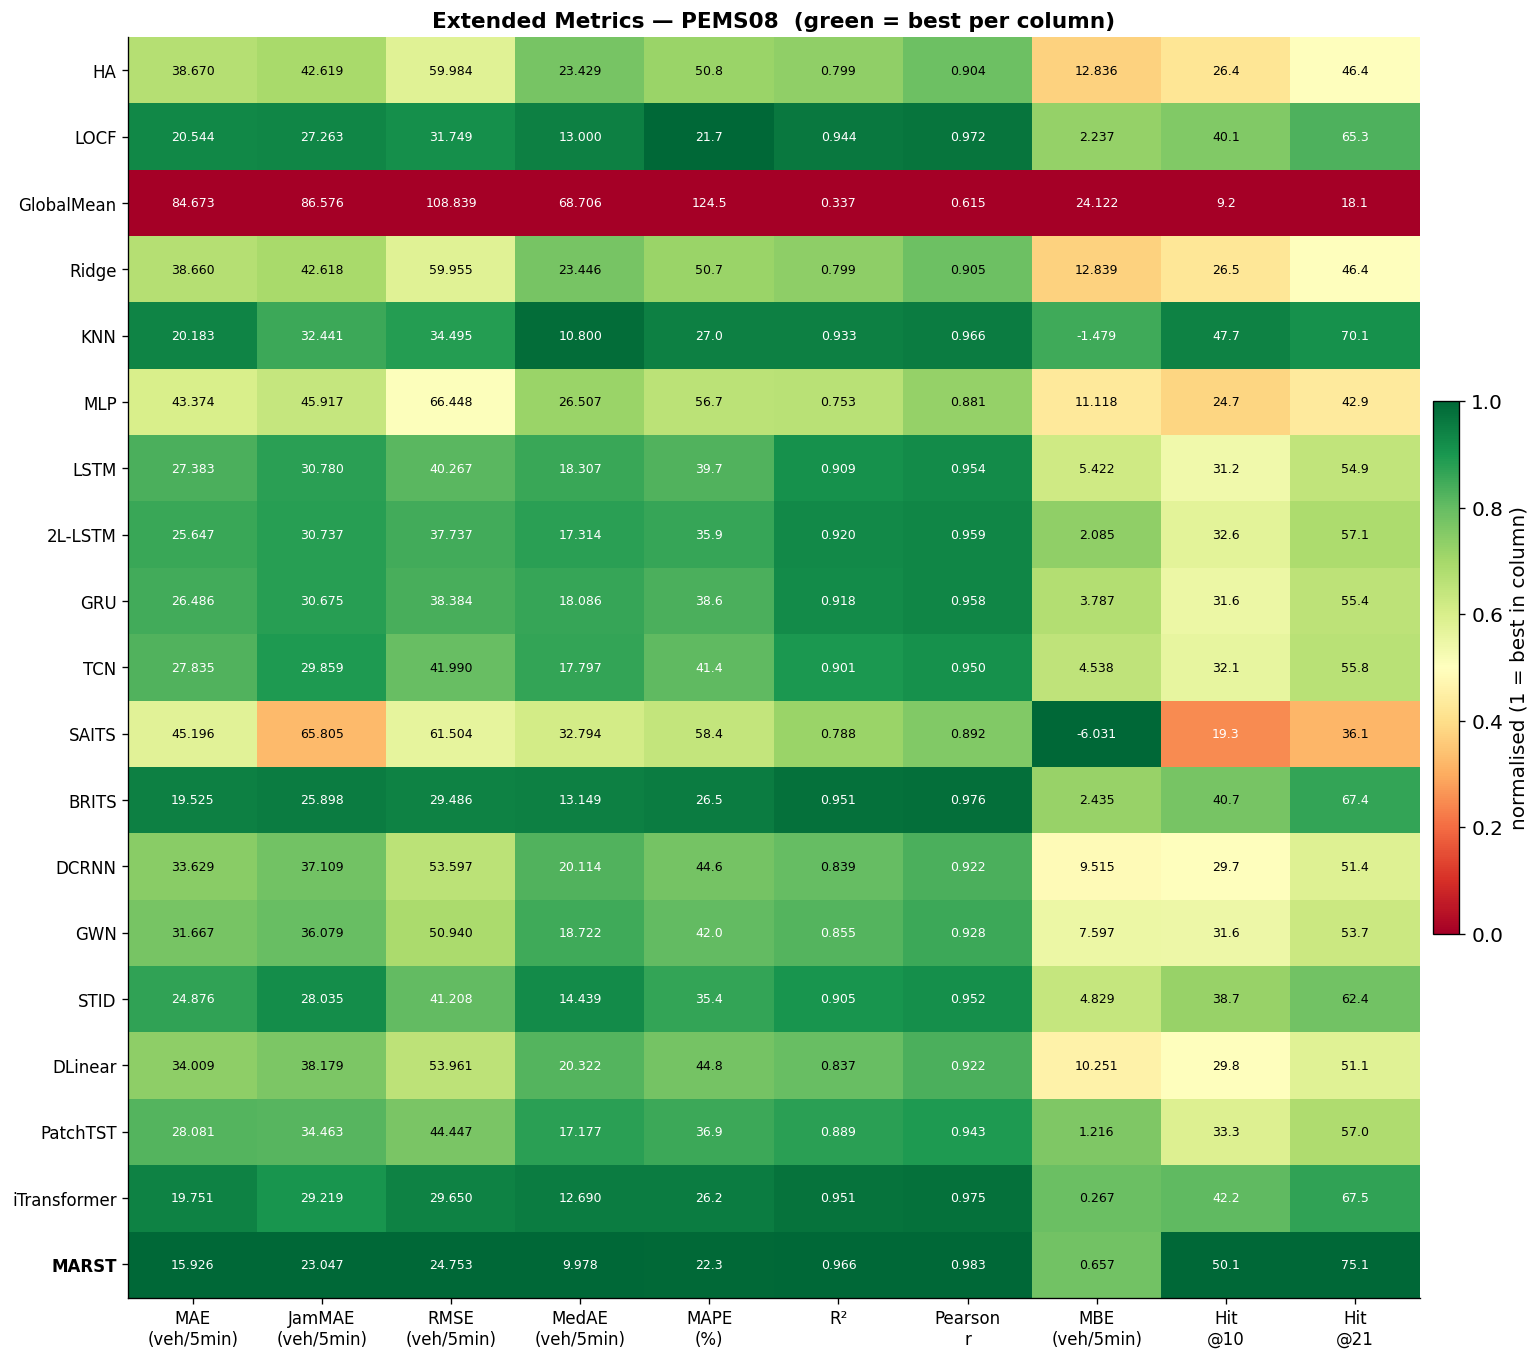
\includegraphics[width=0.95\linewidth]{fig2_metrics_heatmap.png}
\caption{Extended metrics heatmap on PEMS08.  Per-model performance
across MAE, JamMAE, RMSE, MedAE, MAPE\,\%, $R^2$, Pearson, MBE,
Hit@10, Hit@21.  Green = best per column.  \MARST owns the green cell
in every column except MBE.}
\label{fig:heatmap}
\end{figure}

\section{Hyperparameter and Implementation Details}
\label{app:hparams}

\paragraph{Architecture.}  Hidden width $d = 128$; $n_{\text{layers}}
= 6$ STBlocks; $n_{\text{heads}} = 4$; feed-forward expansion 2;
dropout 0.1; GELU activation; PreNorm.  Anchor gate: $L(128, 32) \to
\mathrm{GELU} \to L(32, 3) \to \mathrm{softmax}$.  Residual head:
$L(128, 64) \to \mathrm{GELU} \to L(64, 1)$.  Meta-gate: $L(129, 32)
\to \mathrm{GELU} \to L(32, 1) \to \sigma$ with the bias initialised
so $\alpha \approx 0.05$ at the start of training.  Soft-\LOCF decay:
per-sensor $d_n = \sigma(\ell_n)$, $\ell_n \in \Real^{N}$ a learnable
logit initialised so $d_n \approx 0.95$.

\paragraph{Training.}  Adam with learning rate $1 \times 10^{-3}$;
cosine annealing across the full epoch count; gradient clipping at
norm 0.5; batch size 4 windows; batch time 48 time-steps
($\approx 4$\,h); 800 epochs for the main runs; 400 for the ablation
and decay-sweep variants.  Jam-weight 2$\times$ for cells in the
congested regime.  Load-balance aux loss weight $\lambda = 0.02$.
Sparsity curriculum: training mask ramps from 0.60 to 0.80 over the
first 75\,\% of epochs, then holds at 0.80.

\paragraph{Anti-leak.}  Training window $[0, 4000)$; evaluation window
$[4500, 4950)$; 500-step gap.  Held-out-truth corruption and
future-perturbation tests run after every dataset; verdict
\texttt{NO LEAK / CAUSAL} required for the pipeline to proceed.

\paragraph{Reproducibility.}  Per-thread
\texttt{np.random.default\_rng(train\_seed)} and per-device
\texttt{torch.Generator(device=dev).manual\_seed(train\_seed*31 +
gpu\_id)} for every concurrent training worker.  Both T4 GPUs receive
identical data mirrors via \texttt{.to(device)} no-op copies.  Trained
models are explicitly moved to \texttt{cuda:0} before returning from
the worker so the post-training evaluation code path does not hit a
device-mismatch error.  The reference implementation is
\texttt{marst-learnable-results.ipynb}.

% =============================================================================
\bibliography{references}

\end{document}
